\documentclass[11pt]{article}

\usepackage[margin=1in]{geometry}
\usepackage{amsmath,amssymb,amsthm,mathtools,bm}
\usepackage{booktabs,tabularx,array,multirow}
\usepackage{graphicx}
\usepackage{subcaption}
\usepackage{enumitem}
\usepackage{microtype}
\usepackage{xcolor}
\usepackage[numbers,sort&compress]{natbib}
\usepackage[colorlinks=true,citecolor=blue!55!black,linkcolor=blue!55!black,urlcolor=blue!55!black]{hyperref}
\usepackage[nameinlink,capitalise,noabbrev]{cleveref}

\newtheorem{theorem}{Theorem}[section]
\newtheorem{proposition}[theorem]{Proposition}
\newtheorem{lemma}[theorem]{Lemma}
\newtheorem{corollary}[theorem]{Corollary}
\newtheorem{assumption}[theorem]{Assumption}
\newtheorem{definition}[theorem]{Definition}
\newtheorem{remark}[theorem]{Remark}

\newcommand{\E}{\mathbb E}
\newcommand{\Pp}{\mathbb P}
\newcommand{\R}{\mathbb R}
\newcommand{\KL}{\operatorname{KL}}
\newcommand{\TV}{\operatorname{TV}}
\newcommand{\rank}{\operatorname{rank}}
\newcommand{\tr}{\operatorname{tr}}
\newcommand{\dist}{\operatorname{dist}}
\newcommand{\argmin}{\operatorname*{arg\,min}}
\newcommand{\cD}{\mathcal D}
\newcommand{\cM}{\mathcal M}
\newcommand{\cP}{\mathcal P}
\newcommand{\cL}{\mathcal L}
\newcommand{\cA}{\mathcal A}
\newcommand{\Kw}[2]{\mathfrak K_w\!\left(#1\,\middle\|\,#2\right)}
\newcommand{\wh}{\widehat}
\newcommand{\wt}{\widetilde}
\newcommand{\ip}[2]{\left\langle #1,#2\right\rangle}
\newcommand{\norm}[1]{\left\lVert #1\right\rVert}
\newcommand{\given}{\,\middle|\,}

\title{Population Functional Risk for Tensor--Train Compression\\
of Conditional Generators}
\author{Anonymous authors}
\date{September 2026 working paper}

\begin{document}
\maketitle

\begin{abstract}
Tensor decompositions reduce the storage and arithmetic cost of large conditional generators, but weight-reconstruction error can misrank compressed networks on deployment prompts. We study finite-query estimation of one deployable tensor--train (TT) student under population teacher-relative conditional log-score risk, equivalently conditional KL, with tensorizations and ranks selected by penalized likelihood. On compact, rank-separated, functionally identifiable TT strata, a finite pivot-gauge atlas yields a nonasymptotic oracle bound with approximation error plus \(\{d_\lambda+\log H_\lambda+\log(1/\pi_\lambda)\}/n\), where \(d_\lambda\) is the raw core count minus the TT gauge dimension. A horizontal Assouad construction matches the modelwise \(d_\lambda/n\) term. Under local information-normal and off-chart separation conditions, a dense-teacher construction makes approximation and estimation jointly unavoidable for a fixed resource class. The classical local asymptotic minimax constant on the quotient is \(\tfrac12\tr(G_w I_\pi^{-1})\); it reduces to \(d_\lambda/2\) only for matched query and deployment mixtures under conditional KL\@. Identifiable logistic soft labels and direct access to a feasible teacher give exact-recovery counterexamples, so the black-box lower rate does not transfer universally across access models. We also give a rank-boundary result, an explicit equal-budget TT misordering example, and stability-based same-data capability bands. Synthetic TT-tangent experiments recovered the gauge dimension and the predicted \(d_\lambda/(2n)\) law.
\end{abstract}

\noindent\textbf{Keywords:} conditional density estimation; knowledge distillation; large language models; model selection; quotient manifold; tensor train.

\section{Introduction}
\label{sec:intro}

Consider two tensor--train rank allocations with the same parameter count. The first has the smaller Frobenius reconstruction error for every compressed weight matrix, but removes a direction that is rarely activated and decisive on a safety capability. The second reconstructs the weights less accurately but preserves the teacher's conditional law on deployment prompts. A weight-space criterion necessarily selects the first allocation; a population functional criterion selects the second. This elementary possibility is consequential for large conditional generators because compression is ultimately judged through generated behavior, whereas tensor decompositions are usually fitted and compared through weight or activation reconstruction. Recent empirical work has documented this disconnect for post-training tensor compression~\citep{zagitov2026rethinking,swiftsvd2026}. A remaining statistical question is how to define the population target and intrinsic estimation price when one TT-compressed student must be learned from finitely many teacher queries.

Existing guarantees sharply constrain this question. Classical TT theory characterizes representation, approximation, and smooth fixed-rank geometry~\citep{oseledets2011tt,holtz2012manifolds}. Michel and Nouy's tree-tensor theory gives metric entropy and penalized empirical-risk model selection for general contrasts, with fast rates and near-minimax adaptation developed in bounded least squares~\citep{michel2022tree}. TT completion, recovery, regression, and quantile-regression theory already provides nonasymptotic rates, minimax lower bounds, or asymptotic inference in explicit observation models~\citep{imaizumi2017ttrank,zhou2022ttoi,qinwakin2024ttrecovery,qin2024ttregression,liu2024ttquantile,peng2025ttregression}. Matching low-rank adaptation bounds also extend to frozen nonlinear maps and locally quadratic cross-entropy settings~\citep{arunan2026lora}.

A second line of work concerns the observation channel and the criterion used for compression. Statistical analyses of knowledge distillation explain soft-label variance reduction and give generalization or optimization results in structured student models~\citep{phuong2019distillation,menon2021distillation,xie2026distillation}. Compression-based bounds control a network through its compressed description but do not analyze the present teacher-query experiment~\citep{arora2018compression,lotfi2024compression}. Fisher-, activation-, and KL-weighted matrix methods provide local task-sensitive objectives and calibration-aware rank allocation~\citep{fisherweighted2022,gfwsvd2025,iosvd2026,laser2026,rafft2026,statlora2026}; tensor-regression optimism likewise gives prediction-oriented rank selection for neural-network compression~\citep{shi2026optimism}. Among the primary sources located through 7 September 2026, we did not identify the particular oracle/lower-bound pair for the finite-query, teacher-relative conditional-density experiment on a TT weight quotient studied here. Moreover, a dimension-over-sample-size lower bound cannot be asserted without specifying what is observed from the teacher.

We study a finite-query distillation experiment. An observation consists of a deployment environment, a prompt, and one stochastic response from a fixed teacher conditional law. A candidate \(\lambda\) specifies tensorizations and exact, rank-separated TT strata for the compressed layers. The target is the weighted population conditional Kullback--Leibler divergence \(\cD_w(W,W^0)\), and the approximation error is the best joint risk of one \emph{common} deployable student. Our primary question is whether model selection can attain
\[
 \inf_{\lambda\in\Lambda}
 \left\{A_w^2(\lambda)+
 \frac{d_\lambda+\log H_\lambda+\log(1/\pi_\lambda)}{n}\right\},
 \qquad
 d_\lambda=\text{core parameters}-\text{TT gauge dimensions},
\]
and whether both terms are information-theoretically necessary. This experiment describes black-box or API-limited compression and finite-query distillation. We separately give soft-label and white-box counterexamples showing that the black-box lower bound does not transfer without additional assumptions.

Five issues make the question nonstandard. First, raw TT cores are nonidentifiable: adjacent invertible changes of basis leave the contracted tensor unchanged, so parameter counting overstates dimension. Second, quotient identifiability is not functional identifiability. Frozen network symmetries, dead activations, or unsupported prompts can make the conditional-law map singular even after the TT gauge has been removed. Third, approximation, model selection, and rank recovery interact badly near lower-rank strata, where a fixed-rank manifold loses reach. Fourth, capability certification reuses the prompts that selected ranks and fitted cores; ordinary holdout calibration does not justify this reuse. Finally, Fisher information supplies the local second-order geometry of correctly specified conditional KL\@. It is neither the global estimand nor the generic Hessian of an arbitrary downstream loss.

The analysis proceeds from the oracle theorem to its boundaries and extensions. On compact, separated TT quotient strata equipped with a finite pivot-gauge atlas, localized likelihood entropy is proportional to the gauge-adjusted dimension, and penalized likelihood gives a nonasymptotic oracle inequality. An Assouad hypercube in horizontal coordinates matches its estimation term; under local information-normal and off-chart separation conditions, a dense-teacher family also makes approximation and estimation jointly unavoidable for a fixed resource class. Classical local asymptotic minimax theory, instantiated on the quotient experiment, yields the constant \(\tfrac12\tr(G_w I_\pi^{-1})\). Separate access-model counterexamples show exact recovery from an identifiable logistic soft-label design and zero risk when a feasible teacher parameter is provided directly. Finally, we give a scoped functional-versus-Frobenius misordering result and apply algorithmic stability to simultaneous capabilities evaluated on the same independent prompt clusters used in fitting.

The paper makes five contributions.
\begin{enumerate}[leftmargin=*,label=(C\arabic*)]
    \item \textbf{Population TT oracle inequality.} Under a quantitative rank-separated quotient atlas and likelihood regularity conditions, we prove a finite-sample bound for one selected nonlinear TT student with joint population approximation error and complexity \(d_\lambda+\log H_\lambda+\log(1/\pi_\lambda)\), where \(H_\lambda\) is the atlas size; the TT dimension is calculated on the quotient, regularity factors are displayed, and optimization error is kept explicit.
    \item \textbf{Modelwise lower bounds and local constant.} We prove a \(d_\lambda/n\) lower bound on a regular TT stratum and, under explicit local information-normal and off-chart separation conditions, an \(A_w^2(\lambda)+d_\lambda/n\) lower bound for a fixed-budget teacher family. The quotient instantiation of the classical local asymptotic minimax constant becomes \(d_\lambda/2\) only under matched conditional-KL sampling.
    \item \textbf{Access and adaptation boundaries.} We give soft-label and white-box counterexamples to a universal \(d_\lambda/n\) lower bound, and show that uniform rank recovery is impossible within an \(n^{-1/2}\) functional neighborhood of a lower-rank stratum. We state conditional underfit-gap and overfit-penalty conditions sufficient for consistent penalized rank selection.
    \item \textbf{Functional improvement with correct scope.} We quantify when an anisotropic output metric reverses the ordering induced by Frobenius error and show that functional validation selects the better candidate exponentially fast in its risk gap. This is a strict improvement on a constructed class, not a universal domination claim.
    \item \textbf{Application-level same-data certification.} Adapting classical uniform-stability concentration to a fixed coded family, we give simultaneous capability upper bands valid after fitting and selection, along with a least-cost feasibility guarantee. This secondary corollary does not replace protected-holdout testing when stability is unavailable.
\end{enumerate}

The results are stated for finite or length-truncated outputs and for a concrete nonlinear frozen-prefix/frozen-head block. Extending the constants to a complete transformer requires restricted-Jacobian conditioning, sequence-level tail control, multi-layer chart geometry, and a certified optimization guarantee. We expose these requirements rather than treating them as consequences of parameter count.

\section{Related work and claim boundary}
\label{sec:related}

\paragraph{Tensor trains and statistical low-rank models.}
The TT format and its approximation algorithms are developed by~\citet{oseledets2011tt}; the smooth exact-rank manifold and its gauge structure are analyzed by~\citet{holtz2012manifolds}. Most importantly for our claim boundary, \citet{michel2022tree} establish metric-entropy bounds and penalized empirical-risk model selection for general contrasts on tree tensor networks. Their fast \(C_m/n\) rates and near-minimax adaptive results are developed in bounded least squares, with \(C_m\) based on the number of core entries or nonzero entries rather than the gauge-adjusted manifold dimension. TT-specific statistical theory includes completion error bounds~\citep{imaizumi2017ttrank}, minimax-optimal estimation in a spiked-tensor experiment~\citep{zhou2022ttoi}, noisy sensing and completion guarantees for factorized recovery~\citep{qinwakin2024ttrecovery}, tensor-on-tensor regression upper and lower bounds~\citep{qin2024ttregression}, and regression or quantile-regression rates and inference~\citep{liu2024ttquantile,peng2025ttregression}. More general tangent-space inference and rank-identification results further narrow the claim~\citep{xu2025tensorinference,silva2026rank}.

These works prevent us from claiming priority for a tensor-network oracle, gauge adjustment, TT minimax theory, tensor inference, or rank selection in isolation. Our object is instead the image of a TT weight quotient under a frozen nonlinear conditional-law map. The likelihood metric can collapse relative to the tensor manifold, and approximation is measured after the entire frozen computation. The entropy result below uses an explicit finite pivot atlas on compact rank-separated strata; it is not a global entropy theorem for singular TT varieties.

\paragraph{LLM compression and rank allocation.}
Replacing dense neural-network layers by TT layers predates this work~\citep{novikov2015tensorizing}; performance decompositions for TT neural regression and TT compression of GPT-family embeddings are also established~\citep{qi2020ttdnn,tensorgpt2023}. Thus neither TT neural compression nor its application to language models is new here. Adjacent theory supplies approximation guarantees for matrix low-rank DNN compression and existence guarantees for pruned or quantized wide networks~\citep{zhang2025lowrankcompression,elcheairi2026compression}. Weight-space TT-SVD and higher-order SVD optimize algebraic reconstruction criteria, whose limitations in post-training LLM compression are documented by~\citet{zagitov2026rethinking}. Swift-SVD uses calibration activations and dynamic global allocation~\citep{swiftsvd2026}; Fisher-weighted SVD and GFWSVD use local task-sensitive weights~\citep{fisherweighted2022,gfwsvd2025}.

Especially close to our local geometry, IO-SVD derives an output metric from a second-order top-token KL expansion and performs heterogeneous rank allocation, while LASER derives a curvature-weighted SVD objective using Kronecker-factored Fisher information~\citep{iosvd2026,laser2026}. RAFFT, MetaTT, and StatLoRA likewise adapt ranks or components by optimization and statistical scores~\citep{rafft2026,metatt2025,statlora2026}. These methods occupy loss-aware local geometry and rank allocation; our functional metric and misordering example are therefore not claimed as new compression objectives. They do not, however, establish the finite-query population TT oracle/lower relation studied here. In particular, optimizer-trajectory inference for LoRA components is not inference for a population TT approximation frontier.

\paragraph{Prediction-aware tensor selection.}
The closest tensor-regression collision is~\citet{shi2026optimism}, who derive training--testing optimism for Gaussian random-design CP/Tucker regression and apply a prediction-oriented selector to network compression; they explicitly leave TT optimism as a future direction. Information-theoretic pruning formulates output distortion as a rate--distortion problem~\citep{isik2022pruning}. \citet{haverbeck2026kvcache} give query-distribution population MSE and minimax-optimal upper and lower bounds for fixed-budget KV-cache summaries, with risk governed by response-covariance spectral tails. Matching upper and lower sample-complexity results for well-specified LoRA already cover a frozen nonlinear pretrained map and locally quadratic cross-entropy examples~\citep{arunan2026lora}. We therefore do not claim the first prediction-aware objective, the first population/minimax functional compression theory, the first nonlinear frozen low-rank rate, or the first matching low-rank neural rate. The residual question is narrower: TT weight replacement learned from stochastic teacher queries, teacher-relative conditional KL under new prompts, model selection over quotient strata, and a fixed-budget approximation construction.

\paragraph{Knowledge distillation and teacher access.}
The main experiment is a form of finite-query knowledge distillation. Existing statistical theory shows how a teacher's probability vector can reduce variance and characterizes bias--variance tradeoffs from imperfect teachers~\citep{menon2021distillation}; other analyses give fast generalization for structured distillation models or isolate optimization benefits~\citep{phuong2019distillation,xie2026distillation}. These results make neither teacher-relative KL nor the variance reduction from soft labels a contribution of this paper. Our access result has the more limited purpose of showing that a black-box \(d/n\) lower bound cannot be transferred unchanged to an exact-soft-label experiment. Zero risk follows under white-box access to a feasible teacher and also in the stated full-rank logistic soft-label experiment; these are counterexamples, not a minimax characterization of probability-vector distillation.

\paragraph{Generalization and model selection.}
Compression-based bounds relate description length or perturbation to generalization~\citep{arora2018compression,lotfi2024compression}; classical structural risk minimization and localized empirical-process arguments explain fast likelihood rates~\citep{birge2007massart,koltchinskii2006local}. Likewise, dimension corrections for expected KL risk and sandwich behavior under misspecification are classical~\citep{akaike1973information,white1982misspecified,vandervaart1998}. Our result instantiates this machinery on rank-separated TT quotients and states a modelwise lower experiment under local information-normal and off-chart separation conditions. The code length \(\log(1/\pi_\lambda)\) is used only for a fixed countable candidate family. It is not assigned after inspecting the data, and the local trace constant is presented as a quotient instantiation of classical likelihood theory rather than a new LAN principle.

\paragraph{Risk control after selection.}
Learn-then-Test and Pareto Testing provide simultaneous control with protected calibration data~\citep{angelopoulos2021ltt,laufer2023pareto}, while PAC--Bayes bounds can control multiple error types simultaneously~\citep{adams2024multiple}. Algorithmic stability controls generalization of data-dependent fitted predictors~\citep{bousquet2002stability}, and later work gives sharper high-probability stability bounds~\citep{feldman2019stability,bousquet2020sharper}. Our secondary certificate applies the classical stability-plus-bounded-differences argument and a coded union bound to cluster-level capability losses. We claim no new general concentration method: the contribution is an application-level formulation for a fixed family of TT fitting procedures, and its usefulness depends on a verifiable stability modulus.

\Cref{tab:boundary} summarizes these distinctions and the remaining claim.

\begin{table}[t]
\centering
\caption{Claim boundary relative to the closest families of work.}
\label{tab:boundary}
\small
\begin{tabularx}{\textwidth}{@{}>{\raggedright\arraybackslash}p{.22\textwidth}>{\raggedright\arraybackslash}X>{\raggedright\arraybackslash}X@{}}
\toprule
Work family & Already established & Missing relative to this paper\\
\midrule
TT manifold and statistical theory & Gauge quotient, tangent geometry, fixed-rank dimension, TT rates, and minimax results & Conditional-law visibility in the teacher-query experiment\\
Tree-tensor risk oracles & General-contrast entropy and model selection; fast bounded least-squares rates & TT weights inside a frozen conditional generator and teacher-relative KL\\
Tensor regression/LoRA theory & Prediction-aware selection, nonlinear pretrained maps, and matching low-rank rates & TT quotient under stochastic teacher queries and modelwise dense-teacher approximation\\
Knowledge distillation & Soft-label variance reduction, generalization, and optimization theory & Access comparison restricted to a TT-compressed student class\\
Loss-aware LLM compression & Fisher, activation, KL, or output-sensitive objectives and rank allocation & Nonasymptotic population oracle under an explicit query experiment\\
Multi-risk certification & Simultaneous control, high-probability stability, and structured data reuse & Application to a fixed coded TT algorithm family on prompt clusters\\
This paper & The preceding ingredients are coupled in one conditional experiment & Singular-union TT geometry, full-transformer, and unrestricted-sequence extensions remain open\\
\bottomrule
\end{tabularx}
\end{table}

As of 7 September 2026, the search summarized in this section supports only ``we did not identify,'' not universal absence. The theory would become classical and incremental if reduced to the statement that a smooth \(d\)-dimensional likelihood model has risk \(d/n\). Accordingly, our claim is the coupling of a specified teacher-query experiment with TT quotient coordinates and functional visibility. The entropy theorem is restricted to compact, rank-separated strata with its displayed atlas constants, and the approximation-plus-estimation lower theorem requires the stated local information-normal and off-chart separation conditions; neither is asserted as a global theorem over singular TT unions.

\section{Statistical experiment and population targets}
\label{sec:experiment}

\subsection{Finite-query teacher experiment}

Let \(E\in\{1,\ldots,K\}\) index deployment environments, with prespecified weights \(w_e>0\) and \(\sum_e w_e=1\). Conditional on \(E=e\), a prompt \(X\) has law \(P_e\). The teacher is a fixed conditional distribution
\[
q_0(y\mid x,e)=p_{W^0}(y\mid x,e),
\]
where \(Y\) is a complete response in a finite or length-truncated output space \(\mathcal Y\). The main experiment observes
\begin{equation}
 Z_i=(E_i,X_i,Y_i)\stackrel{\mathrm{iid}}\sim Q_0^w,
 \quad E_i\sim\operatorname{Cat}(w),\quad
 X_i\mid E_i=e\sim P_e,\quad
 Y_i\mid X_i,E_i\sim q_0,
 \label{eq:experiment}
\end{equation}
for \(i=1,\ldots,n\). One response is one statistical unit; tokens within a continuation are not treated as independent observations.

A model index \(\lambda=(\tau,\bm r)\in\Lambda\) specifies tensorizations and TT ranks. It determines a deployable class \(\Theta_\lambda\) and conditional laws \(p_W\), \(W\in\Theta_\lambda\). A fitting routine does not enter \(\lambda\) unless it changes the deployable class; its failure to attain the empirical optimum is recorded as \(\varepsilon_{\lambda,\mathrm{opt}}\).

For two conditional laws \(q\) and \(p\), define the truth-first divergence
\begin{equation}
 \Kw{q}{p}
 =\sum_{e=1}^K w_e\E_{X\sim P_e}
 \KL\{q(\cdot\mid X,e)\|p(\cdot\mid X,e)\}.
 \label{eq:truth-first-kl}
\end{equation}
The order in \cref{eq:truth-first-kl} fixes the asymmetric KL arguments. For a student
parameter \(W\) and teacher parameter \(W^0\), define
\begin{align}
 \cD_e(W,W^0)
 &=\E_{X\sim P_e}\KL\{q_0(\cdot\mid X,e)\|p_W(\cdot\mid X,e)\},\\
 \cD_w(W;W^0)&=\sum_{e=1}^K w_e\cD_e(W,W^0)
 =\Kw{p_{W^0}}{p_W}.
 \label{eq:functional-risk}
\end{align}
This is an exact, global proper-score divergence. No quadratic or Fisher approximation is used in its definition. The joint approximation error of one network is
\begin{equation}
 A_w^2(\lambda)=\inf_{W\in\Theta_\lambda}\cD_w(W,W^0).
 \label{eq:joint-approx}
\end{equation}
In general,
\[
A_w^2(\lambda)\ge
\sum_e w_e\inf_{W_e\in\Theta_\lambda}\cD_e(W_e,W^0),
\]
because the expression on the right is allowed to deploy a different network in each environment.

If calibration proportions \(\pi_e\) differ from \(w_e\), the likelihood contrast is weighted by \(w_e/\pi_e\), and rates depend on \(\max_e w_e/\pi_e\). We take \(\pi=w\) in the main finite-sample theorem and return to general \(\pi\) in the local asymptotic result.

\subsection{Downstream degradation is a separate estimand}

Let \(L_e(y;x,r)\in[0,B_e]\) be a bounded capability loss, possibly depending on a task reference \(r\), and suppose teacher and student generation use their respective conditional laws. Define
\[
\Delta_e(W)=
\E\{L_e(Y_W;X,R)-L_e(Y_0;X,R)\}.
\]
The following transfer is useful but deliberately one-way.

\begin{proposition}[Proper-score to bounded-task transfer]
\label{prop:pinsker-transfer}
For every \(W\),
\[
 |\Delta_e(W)|
 \le B_e\E_{P_e}\TV\{p_W(\cdot\mid X,e),q_0(\cdot\mid X,e)\}
 \le B_e\sqrt{\cD_e(W,W^0)/2}.
\]
Consequently, controlling \(\cD_e\) controls every prespecified bounded randomized-output capability loss. A deterministic argmax decoder requires an additional margin condition and is not covered by this statement.
\end{proposition}

\subsection{Soft-label and white-box access are different experiments}

Under \emph{soft-label query access}, each sampled prompt is accompanied by
the full vector \(q_0(\cdot\mid X_i,E_i)\).  Define the soft-label loss
\[
 \bar\ell_W(X,E)=-\sum_y q_0(y\mid X,E)\log p_W(y\mid X,E).
\]
Write \(\bar\cD_w(\theta)=\Kw{q_0}{p_\theta}\) for its population
divergence, up to the teacher-only entropy constant.
Only prompt quadrature remains random.  This is distinct from
\emph{white-box access}, in which the teacher parameter \(W^0\) itself is
provided directly. The following proposition gives two precise ways in which the
black-box lower bound fails to transfer; it is not a minimax characterization
of every soft-label experiment.

\begin{proposition}[Access-dependent counterexamples and soft-label limit]
\label{prop:access}
Assume a regular coordinate \(\theta\in\R^d\).
\begin{enumerate}[label=(\roman*),leftmargin=*]
    \item Under white-box access, if \(q_0=p_{\theta_0}\) and \(\theta_0\)
    is feasible, the estimator that returns \(\theta_0\) has exactly zero
    population excess risk for every \(n\).
    \item Soft labels alone can also permit finite-sample exact recovery.  In
    binary logistic regression,
    \(q_0(1\mid X)=\sigma(X^\top\theta_0)\), the observed labels satisfy
    \[
      \operatorname{logit}\{q_0(1\mid X_i)\}=X_i^\top\theta_0.
    \]
    If \(n\ge d\) and the design matrix has column rank \(d\), solving this
    linear system recovers \(\theta_0\) exactly and hence gives zero
    population divergence.  Therefore no universal positive \(c d/n\)
    lower bound holds over all soft-label experiments.
    \item More generally, under correct specification the pointwise score
    \(\nabla\bar\ell_{\theta_0}(X,E)\) vanishes, but exact recovery requires
    empirical identifiability and an optimizer or tie-break that selects the
    population law.  Under misspecification, let \(\theta^*\) be an interior
    population minimizer, \(H=\E\nabla^2\bar\ell_{\theta^*}(X,E)\succ0\), and
    \[
      V_X=\operatorname{Var}\{\nabla\bar\ell_{\theta^*}(X,E)\}.
    \]
    Under standard smooth M-estimation conditions, an empirical soft-label minimizer satisfies
    \[
      \sqrt n(\wh\theta-\theta^*)\rightsquigarrow
      N(0,H^{-1}V_XH^{-1}),
      \qquad
      n\E\{\bar\cD_w(\wh\theta)-\bar\cD_w(\theta^*)\}
      \longrightarrow \tfrac12\tr(V_XH^{-1}),
    \]
    whenever the sequence is uniformly integrable. In particular, \(V_X=0\)
    at pointwise correct specification.
\end{enumerate}
\end{proposition}

Under regular matched-information conditions, averaging \(m\) independent teacher draws at each of \(n\) prompts gives a response-noise contribution of order \(d/(nm)\) at correct specification. Prompt-quadrature variation under misspecification need not shrink with \(m\). Greedy teacher outputs are not stochastic draws from \(q_0\), so they do not instantiate \cref{eq:experiment}.

\section{TT quotient geometry and functional identifiability}
\label{sec:geometry}

\subsection{Gauge-adjusted dimension}

For compressed layer \(\ell\), let the prescribed tensorization have mode sizes \(m_{\ell1},\ldots,m_{\ell q_\ell}\) and exact minimal TT ranks
\[
1=r_{\ell0},r_{\ell1},\ldots,r_{\ell,q_\ell-1},r_{\ell q_\ell}=1.
\]
Its cores \(G_{\ell j}\) have shape
\(r_{\ell,j-1}\times m_{\ell j}\times r_{\ell j}\). The gauge group
\[
\mathcal G_\lambda=
\prod_\ell\prod_{j=1}^{q_\ell-1}\mathrm{GL}(r_{\ell j})
\]
acts through
\[
G_{\ell1}\mapsto G_{\ell1}S_{\ell1},\quad
G_{\ell j}\mapsto S_{\ell,j-1}^{-1}G_{\ell j}S_{\ell j},\quad
G_{\ell q_\ell}\mapsto S_{\ell,q_\ell-1}^{-1}G_{\ell q_\ell}.
\]
The contracted tensor is unchanged.

\begin{lemma}[TT quotient dimension]
\label{lem:tt-dimension}
On the exact-minimal-rank stratum, the gauge action is free and the quotient for independent, untied compressed layers is a smooth manifold of dimension
\begin{equation}
d_\lambda=
\sum_\ell\left\{
\sum_{j=1}^{q_\ell}r_{\ell,j-1}m_{\ell j}r_{\ell j}
-\sum_{j=1}^{q_\ell-1}r_{\ell j}^2
\right\}+d_{\lambda,\mathrm{free}},
\label{eq:tt-dim}
\end{equation}
where \(d_{\lambda,\mathrm{free}}\) counts other identifiable free parameters. With tied or shared cores, \cref{eq:tt-dim} must be replaced by the rank of the constrained quotient map.
\end{lemma}

The next result makes the atlas in the oracle theorem concrete. For layer
\(\ell\), put \(N_{\ell j}=\prod_{k\le j}m_{\ell k}\). Let
\(U_{\ell j}(W)\in\R^{N_{\ell j}\times r_{\ell j}}\) be any orthonormal
basis for the column space of the \(j\)th unfolding, put
\(P_{\ell j}(W)=U_{\ell j}(W)U_{\ell j}(W)^\top\), and define
\(c_{\ell j}=\binom{N_{\ell j}}{r_{\ell j}}^{-1/2}\).

\begin{proposition}[Thresholded pivot cover and finite TT atlas]
\label{prop:tt-atlas}
Fix the mode sizes and exact minimal ranks. On the set of tensors satisfying
\(\norm{W}_F\le R\) and
\(\sigma_{r_{\ell j}}\{\operatorname{unfold}_j(W_\ell)\}\ge\eta>0\)
at every internal bond, define for each collection of row sets
\(I=(I_{\ell j})\), \(|I_{\ell j}|=r_{\ell j}\), the basis-invariant patch
\begin{equation}
 \mathcal P_I=\left\{W:
 \lambda_{\min}\{P_{\ell j}(W)[I_{\ell j},I_{\ell j}]\}
 >c_{\ell j}^2/4\ \text{at every internal bond}\right\}.
 \label{eq:pivot-patch}
\end{equation}
These patches cover the separated quotient, and their number is at most
\begin{equation}
 M_\lambda=H_{\lambda,\mathrm{free}}
 \prod_\ell\prod_{j<q_\ell}
 \binom{N_{\ell j}}{r_{\ell j}},
 \label{eq:pivot-count}
\end{equation}
where \(H_{\lambda,\mathrm{free}}=1\) for identifiable free coordinates in a
single compact Euclidean domain. On \(\mathcal P_I\), the normalized interface
\[
 \bar L_{\ell j}^{I}(W)=P_{\ell j}(W)[:,I_{\ell j}]
 \{P_{\ell j}(W)[I_{\ell j},I_{\ell j}]\}^{-1}
\]
is a smooth, basis-independent normalization and satisfies
\(\bar L_{\ell j}^{I}[I_{\ell j},:]=I_{r_{\ell j}}\).

The separated compact quotient has a finite gauge-fixed Euclidean atlas of
dimension \(d_\lambda\) subordinate to these thresholded pivot patches; let
its total size be \(H_\lambda<\infty\). The chart and inverse-chart
derivatives through order two are bounded by
\begin{equation}
 C_{\mathrm{atlas},\lambda}
 =C\bigl((m_{\ell j}),(r_{\ell j}),q_\ell,R,\eta^{-1},
 (c_{\ell j}^{-1})\bigr)<\infty.
 \label{eq:atlas-constant}
\end{equation}
In particular, if \(B_d(a,t)\) lies in one subchart, then
\[
 \log N\{\epsilon,\psi_I(B_d(a,t)),\norm{\cdot}_F\}
 \le d_\lambda\log\left(1+\frac{2C_{\mathrm{atlas},\lambda}t}{\epsilon}\right).
\]
The finite-subatlas extraction does not imply \(H_\lambda\le M_\lambda\): a
pivot patch need not be one global Euclidean chart. Neither \(H_\lambda\) nor
\cref{eq:atlas-constant} is claimed optimal, and both can deteriorate as
\(\eta\downarrow0\).
\end{proposition}

For uniform results, let \(\Theta_\lambda(\eta,R)\) be a compact portion of the quotient on which tensor norms are at most \(R\), every required TT unfolding has smallest nonzero singular value at least \(\eta>0\), and a finite horizontal atlas has condition number at most \(C_{\mathrm{chart}}\). We suppress \((\eta,R)\) below. Lower-rank models are included as separate candidates; we do not silently close an exact-rank stratum by adding its singular boundary.

\subsection{Functional rather than merely tensor identifiability}

Let \(\Phi([W])=p_W(\cdot\mid X,E)\) be the conditional-law map after contraction and frozen-network propagation. At a regular \(W\), write \(T_W^H\Theta_\lambda\) for a horizontal quotient tangent. The conditional-KL pullback is
\begin{equation}
G_w(W)[H,H']
=\sum_e w_e\E_{X\sim P_e,Y\sim p_W}
\{D_W\log p_W(Y\mid X,e)[H]\,
  D_W\log p_W(Y\mid X,e)[H']\}.
\label{eq:functional-metric}
\end{equation}
The \emph{functional dimension} is
\[
d_{\mathrm{fun}}(W)=\rank\{G_w(W)|_{T_W^H\Theta_\lambda}\}\le d_\lambda.
\]
Our gauge-dimensional results require constants \(0<\underline\kappa\le\overline\kappa<\infty\) such that
\begin{equation}
 \underline\kappa\norm{H}_F^2
 \le G_w(W)[H,H]
 \le\overline\kappa\norm{H}_F^2,
 \qquad H\in T_W^H\Theta_\lambda,
\label{eq:restricted-info}
\end{equation}
uniformly on the chart used by the theorem. Without \cref{eq:restricted-info}, \(d_\lambda\) is only an algebraic entropy upper bound; a sharp local rate uses the rank or spectrum of the functional operator.

\subsection{A verifiable nonlinear frozen-network block}

To make \cref{eq:restricted-info} more than an abstract assumption, consider
\begin{equation}
h=h(X,E)\in\R^p,\qquad
z_W=b(X,E)+C\phi(Wh),\qquad
p_W=\operatorname{softmax}(z_W),
\label{eq:nonlinear-block}
\end{equation}
where the prefix \(h\), residual logits \(b\), and head \(C\in\R^{V\times k}\) are frozen, \(\phi\) acts elementwise, and the tensorization of \(W\in\R^{k\times p}\) lies in a TT stratum.

\begin{proposition}[Restricted curvature for a nonlinear block]
\label{prop:block-curvature}
Suppose on the permitted activation range that \(\phi\in C^3\), \(|\phi'|\ge\kappa_\phi>0\), and derivatives up to order three are bounded. Suppose
\[
\E(hh^\top)\succeq\kappa_h I,
\quad \bm 1^\top C=0,
\quad
C^\top\{\operatorname{diag}(p_W)-p_Wp_W^\top\}C\succeq\kappa_C I
\]
uniformly on the model. Then for every ambient perturbation \(H\),
\[
G_w(W)[H,H]\ge
\kappa_C\kappa_\phi^2\kappa_h\norm{H}_F^2.
\]
Consequently the conditional-law map is locally injective on every well-conditioned horizontal TT chart.
\end{proposition}

Local injectivity in this proposition is a property of the student family and
does not depend on the teacher.  Under misspecification, it is instead the
quadratic margin of the teacher-relative cross-entropy that additionally
requires its residual-Hessian perturbation to be smaller than the displayed
model curvature.

The proposition covers a nonlinear compressed block between a frozen prefix and head, not an unrestricted transformer. It also removes the common-softmax-logit direction through the condition on \(C\). Dead prefix directions, unexcited prompts, or additional network symmetries violate its assumptions and reduce functional dimension.

\section{A population functional-risk oracle inequality}
\label{sec:oracle}

\subsection{Candidate fits and selection}

Assign every member of a fixed finite or countable candidate list a code probability \(\pi_\lambda>0\), with \(\sum_{\lambda\in\Lambda}\pi_\lambda\le1\), and write \(x_\lambda=\log(1/\pi_\lambda)\). Split the observations independently into samples of sizes \(n_1\) and \(n_2\). On the first sample, compute an approximate likelihood fit
\begin{equation}
 P_{n_1}\ell_{\wh W_\lambda}
 \le \inf_{W\in\Theta_\lambda}P_{n_1}\ell_W
 +\varepsilon_{\lambda,\mathrm{opt}},
 \qquad \ell_W(Z)=-\log p_W(Y\mid X,E).
 \label{eq:within-fit}
\end{equation}
On the second sample, select
\begin{equation}
 \wh\lambda\in\argmin_{\lambda\in\Lambda}
 \left\{P_{n_2}\ell_{\wh W_\lambda}
       +\kappa_B\frac{x_\lambda}{n_2}\right\}
 \quad\text{up to error }\varepsilon_{\mathrm{sel}},
 \qquad \wh W=\wh W_{\wh\lambda}.
 \label{eq:selector}
\end{equation}
The split makes the fitted candidates fixed during validation. A same-sample version is given in \cref{cor:same-sample-oracle} under a stronger uniform condition.

\subsection{Regularity conditions}

For each \(\lambda\), let \(W_\lambda^*\) be a population KL projection attaining \cref{eq:joint-approx}. We impose the following on the full compact class used for empirical fitting, rather than only along the realized optimization path.

\begin{assumption}[Regular likelihood TT models]
\label{ass:oracle}
There are constants \(B<\infty\) and, for each \(\lambda\), \(\mu_\lambda,L_\lambda>0\) and a finite horizontal atlas of size \(H_\lambda\) such that:
\begin{enumerate}[label=(A\arabic*),leftmargin=*]
    \item \textbf{Likelihood ratios:} \(e^{-B}\le p_W(Y\mid X,E)/q_0(Y\mid X,E)\le e^B\), \(Q_0^w\)-almost surely, for every \(W\) in every fitted class.
    \item \textbf{Projection, local margin, and global gap:} the minimizing conditional law \(p_{W_\lambda^*}\) is unique. It is represented by an interior chart point \(\theta_\lambda^*\), and on a neighborhood \(U_\lambda^*\) within that chart,
    \[
    \cD_w\{\psi_\lambda(\theta),W^0\}-A_w^2(\lambda)
    \ge\frac{\mu_\lambda}{2}\norm{\theta-\theta_\lambda^*}_2^2.
    \]
    For some \(g_\lambda>0\), every \(W\notin U_\lambda^*\) has excess risk at least \(g_\lambda\).
    \item \textbf{Likelihood increments and measurability:} in every chart,
    \[
    |\ell_{\psi_\lambda(\theta)}(z)-
      \ell_{\psi_\lambda(\theta')}(z)|
    \le L_\lambda\norm{\theta-\theta'}_2
    \]
    for almost every \(z\). The loss classes are pointwise measurable and separable.
    \item \textbf{Regular stratum:} \(\Theta_\lambda\) is a compact, gauge-fixed, rank-separated TT stratum covered by the quantitative atlas of \cref{prop:tt-atlas}. Its dimension is \(d_\lambda\) in \cref{eq:tt-dim}.
    \item \textbf{Optimization:} \cref{eq:within-fit,eq:selector} hold with the displayed errors.
\end{enumerate}
\end{assumption}

Assumption~\ref{ass:oracle}(A1) is convenient rather than innocuous. It follows, for example, for a finite output space when teacher and student probabilities are uniformly bounded away from zero. Sequence-level alternatives require subexponential likelihood-ratio control and lead to different constants. The concrete block in \cref{eq:nonlinear-block} supplies the local margin when its restricted curvature remains positive.

\begin{lemma}[Localized quotient entropy]
\label{lem:entropy}
Under Assumption~\ref{ass:oracle}(A1)--(A4), for \(0<u\le1\) and every \(r>0\),
\begin{multline}
\log N\left(
u\sqrt r,
\left\{\ell_W-\ell_{W_\lambda^*}:
W\in\Theta_\lambda,
\ \cD_w(W,W^0)-A_w^2(\lambda)\le r\right\},
L_\infty
\right)\\
\le d_\lambda\log(a_\lambda/u)+\log H_\lambda,
\label{eq:local-entropy}
\end{multline}
where \(a_\lambda\) depends on \(L_\lambda/\sqrt{\mu_\lambda}\), \(g_\lambda^{-1/2}\), compact chart diameters, and atlas conditioning, but not on \(n\). Moreover, for every \(W\in\Theta_\lambda\),
\[
Q_0^w(\ell_W-\ell_{W_\lambda^*})^2
\le v_\lambda
\{\cD_w(W,W^0)-A_w^2(\lambda)\}
\]
with \(v_\lambda=\max\{2L_\lambda^2/\mu_\lambda,4B^2/g_\lambda\}\), after a finite enlargement to cover the boundary of \(U_\lambda^*\).
\end{lemma}

The subtraction of gauge dimensions enters through the Euclidean dimension of a horizontal chart. If the atlas size, reach, or \(L_\lambda^2/\mu_\lambda\) deteriorates with rank, then \(d_\lambda\) alone does not describe the rate constant.

\subsection{Oracle theorem}

\begin{theorem}[Split-sample TT functional oracle]
\label{thm:oracle}
Suppose Assumption~\ref{ass:oracle} holds, \(n_1\wedge n_2\ge2\), and the empirical-process constants implied by \cref{eq:local-entropy} are finite. There are constants \(C_B,C>0\), and regularity factors \(C_{\mathrm{reg},\lambda}\) polynomial in \(a_\lambda\), \(v_\lambda\), and chart conditioning, such that if \(\kappa_B\) is sufficiently large, then for every \(t\ge1\), with probability at least \(1-Ce^{-t}\),
\begin{align}
\cD_w(\wh W,W^0)
\le C_B\inf_{\lambda\in\Lambda}\bigg[&A_w^2(\lambda)
+C_{\mathrm{reg},\lambda}
\frac{d_\lambda+\log H_\lambda+x_\lambda+t}{n_1}
+\frac{x_\lambda+t}{n_2}
+\varepsilon_{\lambda,\mathrm{opt}}\bigg]
+C_B\varepsilon_{\mathrm{sel}}.
\label{eq:oracle-hp}
\end{align}
If \(n_1\asymp n_2\asymp n\), all regularity factors and \(\log H_\lambda\) are uniformly bounded, the risk is bounded, and optimization errors are zero, then
\begin{equation}
\E\cD_w(\wh W,W^0)
\le C\inf_{\lambda\in\Lambda}
\left\{A_w^2(\lambda)+
\frac{d_\lambda+\log(1/\pi_\lambda)}{n}\right\}
+\frac Cn.
\label{eq:oracle-expectation}
\end{equation}
The stochastic term is capped by the maximum allowed KL risk when \(d_\lambda\gtrsim n\).
\end{theorem}

The theorem is a population result: \(A_w^2(\lambda)\) and the left side are evaluated under new deployment prompts. It is also a statement about a statistical optimizer. It does not imply that TT-SVD or unconstrained SGD attains \(\varepsilon_{\lambda,\mathrm{opt}}=0\).

\begin{corollary}[Same-sample structural risk minimization]
\label{cor:same-sample-oracle}
Suppose that, simultaneously over the full coded union, the likelihood-ratio classes satisfy the isomorphic inequality
\[
 |(P_n-P_0)\log(q_0/p_W)|
 \le \tfrac14\cD_w(W,W^0)
 +C\frac{d_\lambda+\log H_\lambda+x_\lambda+t}{n}.
\]
Then a single-sample penalized empirical likelihood with penalty at least a sufficiently large multiple of \((d_\lambda+\log H_\lambda+x_\lambda)/n\) obeys \cref{eq:oracle-hp} with \(n_1=n\) and no validation split.
\end{corollary}

The stronger premise is obtainable from localized entropy and likelihood-ratio Bernstein control, but it must hold over the predeclared union. A path of ranks generated after viewing the same data is not entitled to a post hoc \(\log|\Lambda|\) penalty.

\section{Matching lower bounds, sharp constants, and rank boundaries}
\label{sec:lower}

\subsection{A horizontal Assouad construction}

Let \(h_w\) denote Hellinger distance between the joint laws with the common environment--prompt marginal and the indicated conditional response laws. Fix a regular point in a separated TT stratum and a \(C^2\) horizontal chart
\(\psi:B_d(0,\rho)\to\Theta_\lambda\), where \(d=d_\lambda\).

\begin{assumption}[Local experimental and target metrics]
\label{ass:lower-metric}
For constants \(c_h,C_K>0\) and all \(u,v\in B_d(0,\rho)\),
\begin{align}
h_w^2\{p_{\psi(u)},p_{\psi(v)}\}&\ge c_h\norm{u-v}_2^2,\label{eq:hell-lower}\\
\KL\{Q_{\psi(u)}^w\|Q_{\psi(v)}^w\}&\le C_K\norm{u-v}_2^2.\label{eq:kl-upper}
\end{align}
\end{assumption}

These inequalities follow on a sufficiently small chart from a uniformly nondegenerate conditional information matrix. Their dimension is \(d_\lambda\) because the chart is horizontal; a packing of raw cores would incorrectly count gauge copies.

\begin{theorem}[Gauge-dimensional minimax lower bound]
\label{thm:lower}
Under Assumption~\ref{ass:lower-metric}, for a constant \(c>0\) depending only on \(c_h,C_K\),
\begin{equation}
\inf_{\wt p=\wt p(Z_1,\ldots,Z_n)}\sup_{u\in B_d(0,\rho)}
\E_u\Kw{p_{\psi(u)}}{\wt p}
\ge c\left(\rho^2\wedge\frac{d_\lambda}{n}\right).
\label{eq:lower-dn}
\end{equation}
The infimum is over all conditional-distribution estimators measurable with
respect to the displayed \(n\)-query experiment and not to any additional
teacher information.  Thus the result also holds for estimators constrained
to TT networks.
\end{theorem}

The modelwise rate in \cref{eq:lower-dn} concerns the stochastic-query
experiment and does not apply after the teacher observation channel is changed.

\subsection{Adding irreducible compression error}

A fixed-stratum result does not by itself lower-bound an arbitrary oracle over
a union: a larger unpenalized class could contain the teacher.  The
appropriate approximation statement fixes a resource class and constructs a
dense teacher normal to it.  We next give conditions under which that
construction actually exists.

Let \(\mathcal U\subset\R^D\) be an open dense-block parameter chart and let
\(p_\zeta\), \(\zeta\in\mathcal U\), be its conditional laws.  A separated TT
chart is represented by a \(C^3\) embedding
\[
 \iota:B_d(0,2\rho_0)\longrightarrow\mathcal U,
 \qquad d=d_\lambda<D,
\]
whose image is the local part of \(\Theta_\lambda\).  Write
\[
 J_w(\zeta)=\sum_e w_e\E_{P_e,p_\zeta}
 \{s_\zeta s_\zeta^\top\},
 \qquad s_\zeta=\nabla_\zeta\log p_\zeta(Y\mid X,e).
\]
For an arbitrary teacher conditional \(q\), use the notation
\[
A_w^2(\lambda;q)=\inf_{W\in\Theta_\lambda}\Kw{q}{p_W}.
\]

\begin{proposition}[Smooth Fisher-normal TT tube]
\label{prop:normal-tube}
Suppose \(\rho_0\) has been chosen sufficiently small that the closed chart
below lies in one regular neighborhood. Suppose the dense-block model has common conditional support, its log
densities have three derivatives dominated uniformly on a neighborhood of
\(\iota\{B_d(0,2\rho_0)\}\), and
\[
 \underline\kappa I_D\preceq J_w(\zeta)
 \preceq\overline\kappa I_D
\]
there.  Suppose the singular values of \(D\iota(u)\) are bounded above and
away from zero and the first three derivatives of \(\iota\) are bounded.
Let \(N(u)\) be a \(C^2\) normal field satisfying
\begin{equation}
 D\iota(u)^\top J_w\{\iota(u)\}N(u)=0,
 \qquad
 N(u)^\top J_w\{\iota(u)\}N(u)=1,
 \label{eq:fisher-normal}
\end{equation}
with bounded first two derivatives.  Such a field exists after shrinking a
ball whenever the functional codimension is positive; equivalently, the
profiled normal Hessian is the positive Schur complement of the tangent
information block.  For
\[
 \zeta_{u,a}=\iota(u)+aN(u),\qquad P_{u,a}=p_{\zeta_{u,a}},
\]
assume additionally that the rest of the compact resource class is separated:
there is \(g_0>0\) such that, for all sufficiently small \(a\),
\begin{equation}
 \inf_{u\in B_d(0,\rho_0)}
 \inf_{W\in\Theta_\lambda\setminus
 \iota\{B_d(0,2\rho_0)\}}
 \Kw{P_{u,a}}{p_W}\ge g_0.
 \label{eq:off-chart-gap}
\end{equation}
Put \(\rho=\rho_0/4\). Then there are \(a_0>0\) and constants
\(0<c_T<C_T<\infty\) such that, for
\(u\in B_d(0,\rho)\), \(v\in B_d(0,2\rho_0)\), and
\(0\le a\le a_0\),
\begin{align}
 c_T\{a^2+\norm{u-v}_2^2\}
 &\le \Kw{P_{u,a}}{p_{\iota(v)}}
 \le C_T\{a^2+\norm{u-v}_2^2\},
 \label{eq:tube-loss}\\
 \KL\{(Q_{u,a}^w)^{\otimes n}\|(Q_{v,a}^w)^{\otimes n}\}
 &\le nC_T\norm{u-v}_2^2,
 \label{eq:tube-kl}\\
 c_Ta^2\le A_w^2(\lambda;P_{u,a})&\le C_Ta^2.
 \label{eq:tube-approx}
\end{align}
Here \(Q_{u,a}^w\) has the fixed environment--prompt marginal and conditional
law \(P_{u,a}\).  The off-chart condition is indispensable: local reach alone
does not rule out a second, distant TT representation with smaller functional
risk.
\end{proposition}

The curvature conditions of Proposition~\ref{prop:block-curvature}, applied in
the ambient dense block, verify the information assumption in
Proposition~\ref{prop:normal-tube}.  The codimension condition excludes a TT
class that already fills the dense parameter chart.

\begin{theorem}[Approximation plus estimation under a fixed budget]
\label{thm:tube-lower}
Under Proposition~\ref{prop:normal-tube}, for every fixed
\(0\le a\le a_0\), let \(\mathfrak E_n(\Theta_\lambda)\) denote the measurable
maps from the \(n\)-query sample into \(\Theta_\lambda\). Then
\begin{equation}
\inf_{\wt W\in\mathfrak E_n(\Theta_\lambda)}
\sup_{u\in B_d(0,\rho)}
\E_{u,a}\Kw{P_{u,a}}{p_{\wt W}}
\ge c\left\{a^2+
\left(\rho^2\wedge\frac{d_\lambda}{n}\right)\right\}.
\label{eq:tube-lower-result}
\end{equation}
In view of \cref{eq:tube-approx}, this is equivalent up to constants to
approximation error plus \(d_\lambda/n\) in the local regime for the fixed
resource class \(\Theta_\lambda\). More precisely, it establishes sharpness,
up to constants, of the irreducible approximation term and the within-class
gauge-dimensional estimation term for this teacher family. It neither
lower-bounds the atlas or coding penalties \(\log H_\lambda\) and
\(\log(1/\pi_\lambda)\), nor gives an oracle lower bound over a union that may
contain larger free models.
\end{theorem}

\subsection{A Gaussian-sequence approximation benchmark}

The preceding fixed-budget theorem is the compression lower bound used in the
paper.  For comparison with the final synthetic experiment, consider the
separate Gaussian sequence experiment
\begin{equation}
 Z_j=\theta_j+n^{-1/2}\xi_j,\qquad
 \xi_j\stackrel{\mathrm{iid}}\sim N(0,1),\qquad j\ge1,
 \label{eq:gaussian-sequence}
\end{equation}
under squared \(\ell_2\) loss, and define the approximation class
\[
 \mathcal H_s(L)=\left\{\theta\in\ell_2:
 \sum_{j>D}\theta_j^2\le L^2D^{-2s}
 \text{ for every integer }D\ge1\right\}.
\]

\begin{proposition}[Matching-rate Gaussian-sequence benchmark]
\label{cor:scale}
For every \(s,L>0\), constants \(0<c_s<C_s<\infty\) satisfy
\[
 c_s\inf_{D\ge1}\left\{L^2D^{-2s}+\frac Dn\right\}
 \le
 \inf_{\wt\theta}\sup_{\theta\in\mathcal H_s(L)}
 \E_\theta\norm{\wt\theta-\theta}_2^2
 \le
 C_s\inf_{D\ge1}\left\{L^2D^{-2s}+\frac Dn\right\}.
\]
The upper bound is attained, up to constants, by truncation at the optimizing
\(D\).  An unbounded candidate grid \(1=d_1<d_2<\cdots\) with uniformly
bounded adjacent ratios yields the same rate, up to a grid-dependent constant,
with the infimum restricted to that grid. This proposition is a
matching-rate benchmark for \cref{eq:gaussian-sequence}; transferring it to a growing
conditional-generator experiment requires a separate uniform LAN or
nonasymptotic embedding argument and is not claimed here.
\end{proposition}

\subsection{Local asymptotic minimax constant}

Allow the query environment mixture \(\pi\) to differ from deployment weights \(w\). Let \(I_\pi\) be the information in one query in horizontal coordinates. Let a twice differentiable target divergence satisfy
\[
\cL_w\{p_{\psi(\theta)},p_{\psi(\theta+t)}\}
=\tfrac12t^\top G_wt+o(\norm{t}^2).
\]

\begin{theorem}[Sharp local constant]
\label{thm:lan}
Suppose the horizontal experiment at \(\psi(0)\) is differentiable in
quadratic mean and locally asymptotically normal, \(I_\pi\succ0\) and
\(G_w\succ0\), and the loss expansion is locally uniform.  Assume also local
coercivity: outside every sufficiently small coordinate neighborhood the
target loss is bounded away from zero, uniformly for true parameters in a
smaller neighborhood.  More explicitly, require that for every
\(M,R<\infty\),
\[
\sup_{\norm{h}\vee\norm{b}\le R}
\left|\min\left[M,n\cL_w
 \{p_{\psi(h/\sqrt n)},p_{\psi(b/\sqrt n)}\}\right]
-\min\left[M,\tfrac12(b-h)^\top G_w(b-h)\right]\right|
\longrightarrow0,
\]
and estimators leaving the local chart cannot have smaller limiting truncated
risk.  Then
\begin{equation}
\lim_{R\to\infty}\liminf_{n\to\infty}
\inf_{\wt W_n}\sup_{\norm{h}\le R}
n\E_{\psi(h/\sqrt n)}
\cL_w\{\psi(h/\sqrt n),\wt W_n\}
\ge\frac12\tr(G_wI_\pi^{-1}).
\label{eq:lan-constant}
\end{equation}
An efficient quotient estimator attains equality if it is asymptotically
linear uniformly on compact local alternatives and its rescaled quadratic
losses are uniformly integrable. For correctly specified conditional KL,
\(G_w=I_w\). If \(w=\pi\), the constant is \(d_\lambda/2\); otherwise it is
\(\tfrac12\tr(I_wI_\pi^{-1})\), not \(d_\lambda/2\).
\end{theorem}

Thus \cref{eq:lan-constant} is a lower bound for the local quotient experiment;
equality additionally requires the stated efficiency and uniform-integrability
conditions.

\begin{proposition}[Misspecified excess-target constant]
\label{prop:misspecified-constant}
Let
\[
R_w(\theta)=\Kw{q_0}{p_{\psi(\theta)}}
\]
have an interior stationary minimizer \(\theta^*\) and Hessian
\(G_w=\nabla^2R_w(\theta^*)\succ0\). Suppose an estimator based on queries
from mixture \(\pi\) is asymptotically linear for an estimating function
\(\varphi_\pi\) satisfying
\[
\E_\pi\varphi_\pi(Z,\theta^*)=0,\qquad
H_\pi=\E_\pi\nabla_\theta\varphi_\pi(Z,\theta^*)
=H_\pi^\top\succ0,\qquad
V_\pi=\operatorname{Var}_\pi\{\varphi_\pi(Z,\theta^*)\},
\]
so that
\[
\sqrt n(\wh\theta-\theta^*)\rightsquigarrow
N(0,H_\pi^{-1}V_\pi H_\pi^{-1}).
\]
If the target-risk Taylor remainder and the rescaled losses are uniformly
integrable, then
\begin{equation}
n\E\{R_w(\wh\theta)-R_w(\theta^*)\}
\longrightarrow
\tfrac12\tr\{G_wH_\pi^{-1}V_\pi H_\pi^{-1}\}.
\label{eq:misspecified-constant}
\end{equation}
The ordinary-likelihood projection under \(\pi\) need not minimize the target
risk under \(w\); the proposition therefore requires the displayed
common centering. Importance-weighted likelihood is one way to enforce it.
At correct conditional specification under matched sampling,
\(G_w=H_\pi=V_\pi=I_w\), recovering \(d_\lambda/2\).
\end{proposition}

Thus at a misspecified projection the estimating Hessian and score covariance
generally differ, and the constant in \cref{eq:misspecified-constant} is
sandwich-shaped. This is
another reason not to label every functional matrix ``Fisher.''

\subsection{The lower-rank boundary}

For this subsection take the query and target environment mixtures to agree,
\(\pi=w\), so that the Hellinger and conditional-KL separations below use the
same population mixture.

Let \(\mathcal B_{\bm r}\) be the union of strata strictly below \(\bm r\), and define the gauge-invariant functional separation
\[
\delta_{\bm r}(W)=\inf_{V\in\mathcal B_{\bm r}}
h_\pi(Q_W,Q_V).
\]

\begin{theorem}[No uniform rank recovery at the boundary]
\label{thm:rank-impossibility}
Suppose \(W_0\in\mathcal B_{\bm r}\) has minimal TT rank \(\bm r_0\), and
\(W_t\) lies in the exact-rank \(\bm r\) stratum with \(W_t\to W_0\) and
\[
\KL(Q_{W_0}^\pi\|Q_{W_t}^\pi)\le C\delta_t^2,
\qquad \delta_t=h_\pi(Q_{W_0},Q_{W_t}).
\]
For every rank selector \(\wh{\bm r}\),
\[
\max\left\{
\Pp_{W_0}(\wh{\bm r}\ne\bm r_0),
\Pp_{W_t}(\wh{\bm r}\ne\bm r)
\right\}
\ge\frac{1-\sqrt{Cn\delta_t^2/2}}{2}.
\]
Therefore rank recovery is not uniformly consistent when \(\delta_t=o(n^{-1/2})\), and its error stays bounded away from zero at a sufficiently small constant multiple of \(n^{-1/2}\).
\end{theorem}

Prediction-risk adaptation does not require exact rank recovery. Conversely,
exact recovery requires separation. A natural separated class on which to
seek recovery is
\[
\Theta(\bm r,\eta)=\{W:\operatorname{rank}_{TT}(W)=\bm r,
\ \delta_{\bm r}(W)\ge\eta,\ \text{bounded regularity constants}\}.
\]
Under uniform likelihood-gap deviations of order
\(\{d_{\bm r}+\log(|\Lambda|/\alpha)\}/n\), a transparent sufficient
underfit condition is
\[
\inf_{V\in\mathcal B_{\bm r}}\Kw{p_W}{p_V}
\ge C\frac{d_{\bm r}+\log(|\Lambda|/\alpha)}{n}.
\]
The next elementary proposition records exactly what is additionally needed
for a consistency claim.

\begin{proposition}[Conditional sufficient rank-selection conditions]
\label{prop:rank-sufficiency}
Let \(\Lambda\) be finite, let the teacher \(W\) have minimal candidate rank
\(\bm r\), and define
\[
 \wh{\bm r}\in\argmin_{\bm s\in\Lambda}
 \left\{\inf_{V\in\Theta_{\bm s}}P_n\ell_V
       +\frac{\operatorname{pen}_{\bm s}}n\right\}.
\]
Partition the other candidates into underfit models \(\mathcal U_{\bm r}\)
that do not contain the teacher law and overfit models
\(\mathcal O_{\bm r}\) that do.  Suppose that, on events whose probabilities
tend to one,
\begin{align*}
 \inf_{V\in\Theta_{\bm s}}P_n(\ell_V-\ell_W)&\ge g_n/2,
 &&\bm s\in\mathcal U_{\bm r},\\
 P_n\ell_W-\inf_{V\in\Theta_{\bm s}}P_n\ell_V&\le b_{\bm s,n}/n,
 &&\bm s\in\mathcal O_{\bm r}.
\end{align*}
If eventually
\begin{align*}
 ng_n/2+\operatorname{pen}_{\bm s}-
 \operatorname{pen}_{\bm r}&>0,
 &&\bm s\in\mathcal U_{\bm r},\\
 \operatorname{pen}_{\bm s}-\operatorname{pen}_{\bm r}
 &>b_{\bm s,n},
 &&\bm s\in\mathcal O_{\bm r},
\end{align*}
then \(\Pp_W(\wh{\bm r}=\bm r)\to1\).
\end{proposition}

A population underfit gap
\(g_n\le\inf_{\bm s\in\mathcal U_{\bm r}}
\inf_{V\in\Theta_{\bm s}}\Kw{p_W}{p_V}\), together with uniform deviations
that are \(o(g_n)\), verifies the first event.  Because
\(\Kw{p_W}{p_V}\ge h_\pi^2(Q_W,Q_V)\), the regime
\(\eta_n\sqrt{n/(d_{\bm r}+\log|\Lambda|)}\to\infty\) is a transparent
underfit-separation condition under the displayed deviation scale.  It is not
by itself sufficient for rank consistency: the overfit-gain bounds must also
be proved.  In regular nested models a BIC-type penalty can dominate those
gains, whereas a fixed AIC-type penalty generally does not; near singular TT
strata this domination requires a separate analysis.  We do not claim that
the displayed separation is a universal necessary boundary.

\section{Functional selection, metric misordering, and the role of Fisher}
\label{sec:misordering}

The oracle result is useful only if functional risk can select differently from cheaper algebraic surrogates. We now give a local result that quantifies when this happens.

Let \(Q\succ0\) be the quadratic metric used by a reconstruction rule on a feasible compression-error span \(\mathcal C\); Frobenius error corresponds to \(Q=I\). Fix a regular limiting teacher \(W_*\), let \(G_w(W_*)\succ0\) be the conditional-KL pullback on the same span, and denote the smallest and largest generalized eigenvalues of \((G_w(W_*),Q)\) by \(\lambda_L<\lambda_H\), with \(Q\)-orthonormal generalized eigenvectors \(v_L,v_H\).

\begin{theorem}[Strict local metric misordering]
\label{thm:misordering}
Suppose \(W^0(t)\to W_*\) is a teacher family and two equal-resource compression paths have errors
\[
\delta_A(t)=W_A(t)-W^0(t)=ta v_H+O(t^2),\qquad
\delta_B(t)=W_B(t)-W^0(t)=tb v_L+O(t^2),
\]
where \(0<a<b\) and \(\lambda_Ha^2>\lambda_Lb^2\). If conditional KL is three times continuously differentiable on the paths, then for all sufficiently small \(t>0\),
\begin{align*}
\delta_A(t)^\top Q\delta_A(t)&<\delta_B(t)^\top Q\delta_B(t),\\
\cD_w\{W_A(t);W^0(t)\}&>
\cD_w\{W_B(t);W^0(t)\}.
\end{align*}
Thus the \(Q\)-reconstruction rule selects \(A\), whereas population functional risk selects \(B\). The ratio of the two selected risks can approach the metric condition number \(\lambda_H/\lambda_L\).
\end{theorem}

The path premise is essential: anisotropy somewhere in parameter space does not imply that a particular set of feasible decompositions contains the required directions.  The following construction verifies feasibility rather than assuming it.

\begin{proposition}[Equal-budget rank-one TT realization]
\label{prop:tt-misordering-paths}
Let \(T_H,T_L\) be Frobenius-orthonormal rank-one TT tensors of the same mode
shape.  In the binary conditional model
\[
 p_W(1\mid X)=\sigma\{\langle W,X\rangle\},\qquad
 \Pp(X=T_j)=\rho_j>0,\quad j\in\{H,L\},\qquad \rho_H+\rho_L=1,
\]
take a dense teacher
\(W^0(t)=t(aT_H+bT_L)\) and two equal-budget rank-one students
\(W_A(t)=tbT_L\) and \(W_B(t)=taT_H\).  If \(0<a<b\) and
\(\rho_Ha^2>\rho_Lb^2\), then for all sufficiently small \(t>0\),
\[
 \norm{W_A(t)-W^0(t)}_F^2<\norm{W_B(t)-W^0(t)}_F^2,
 \qquad
 \cD_w\{W_A(t);W^0(t)\}>\cD_w\{W_B(t);W^0(t)\}.
\]
If the left and right factors of \(T_H,T_L\) are linearly independent across
at least one TT cut, then \(W^0(t)\) has TT rank two for \(t>0\), whereas both
students have TT rank one. Thus this moving-teacher local family instantiates
\cref{thm:misordering} inside an explicit TT compression problem with the same
student storage budget.
\end{proposition}

\begin{corollary}[Finite-query selection advantage]
\label{cor:selection-gap}
Let \(W_A,W_B\) be fixed before validation, either prespecified or fitted on an independent first split. Let \(\gamma=\cD_w(W_A,W^0)-\cD_w(W_B,W^0)>0\), and suppose \(|\log(q_0/p_{W_j})|\le B\) for \(j=A,B\). Validation likelihood selects \(B\) with probability at least
\[
1-\exp\{-n_2\gamma^2/(8B^2)\}.
\]
For the class in \cref{thm:misordering}, the Frobenius rule selects \(A\) deterministically. Hence functional validation gives a strict population-risk improvement on this class and identifies the better candidate exponentially fast in the squared risk gap.
\end{corollary}

\subsection{Conditional KL has a local Fisher pullback}

At a correctly specified regular point with horizontal coordinate \(\theta\), the score identity gives
\begin{equation}
\cD_e(\theta+u,\theta)
=\tfrac12u^\top I_e(\theta)u+O(\norm{u}^3),
\qquad
I_e(\theta)=\E_{p_\theta}(s_\theta s_\theta^\top).
\label{eq:fisher-local}
\end{equation}
This classical identity explains Fisher-weighted compression locally. It does not turn the global divergence in \cref{eq:functional-risk} into a quadratic form, and we do not treat the identity itself as a new contribution.

For an ordinary population task loss \(R_e\),
\begin{equation}
R_e(W^0+\delta)-R_e(W^0)
=\nabla R_e(W^0)^\top\delta
+\tfrac12\delta^\top H_e(W^0)\delta
+O(\norm{\delta}^3).
\label{eq:task-expansion}
\end{equation}
The first-order term disappears only under an explicit stationarity condition. Moreover, \(H_e\) need not equal an information matrix. We therefore reserve ``Fisher'' for \cref{eq:fisher-local}, use ``conditional-KL pullback'' for \cref{eq:functional-metric}, and call the general matrix in \cref{eq:task-expansion} a task-risk Hessian.

\section{Secondary result: same-data multi-capability certification}
\label{sec:certification}

The oracle theorem chooses a network by conditional log-score risk, equivalently conditional KL\@. Deployment may additionally require simultaneous capability constraints. We permit reuse of the fitting data, but pay for it through algorithmic stability.

Let \(C_1,\ldots,C_G\) be identically distributed independent prompt clusters; dependence within a cluster is unrestricted. Each cluster contains enough prespecified randomness or paired teacher/student evaluations to form a cluster-level statistic
\(H_e(W;C_g)\) for capability \(e\in\{1,\ldots,K\}\).  Uniformly over \(W\) and \(c\), \(H_e(W;c)\) lies in one common interval of length \(M_e\), and
\[
\Delta_e(W)=\E H_e(W;C).
\]
For every member of a fixed coded family, let \(\mathsf A_\lambda(S)\) be the complete deterministic core-fitting algorithm applied to \(S=(C_1,\ldots,C_G)\). A randomized algorithm is permitted if the stability condition below holds uniformly conditional on one external random seed. Define
\[
\wh\Delta_e(\lambda)=\frac1G\sum_{g=1}^G
H_e\{\mathsf A_\lambda(S);C_g\}.
\]

\begin{assumption}[Replace-one-cluster stability]
\label{ass:stability}
If \(S,S'\) differ in one cluster, then for every evaluation cluster \(c\),
\[
\left|H_e\{\mathsf A_\lambda(S);c\}
-H_e\{\mathsf A_\lambda(S');c\}\right|
\le\beta_{e\lambda}.
\]
\end{assumption}

\begin{theorem}[Simultaneous same-data capability band]
\label{thm:certificate}
Under Assumption~\ref{ass:stability}, assign candidate codes \(\pi_\lambda\) with \(\sum_\lambda\pi_\lambda\le1\), and let
\begin{equation}
 r_{e\lambda}(\alpha)=
 \beta_{e\lambda}+
 (2G\beta_{e\lambda}+M_e)
 \sqrt{\frac{\log\{2K/(\alpha\pi_\lambda)\}}{2G}}.
 \label{eq:stability-radius}
\end{equation}
Then, with probability at least \(1-\alpha\), simultaneously for every \(e\) and \(\lambda\),
\begin{equation}
\left|\Delta_e\{\mathsf A_\lambda(S)\}
-\wh\Delta_e(\lambda)\right|
\le r_{e\lambda}(\alpha).
\label{eq:sim-band}
\end{equation}
Consequently \(U_e(\lambda)=\wh\Delta_e(\lambda)+r_{e\lambda}(\alpha)\) remains a valid upper bound after any data-dependent selection from the fixed coded family.
\end{theorem}

Given tolerances \(\epsilon_e\), define the empirically certified set
\[
 \wh\Lambda_{\mathrm{safe}}
 =\{\lambda:U_e(\lambda)\le\epsilon_e\ \text{for every }e\}.
\]
When \(\wh\Lambda_{\mathrm{safe}}\ne\varnothing\), define the least-cost
certified choice
\begin{equation}
 \wh\lambda_{\mathrm{safe}}
 \in\argmin_{\lambda\in\wh\Lambda_{\mathrm{safe}}}
 \operatorname{Cost}(\lambda).
\label{eq:safe-selector}
\end{equation}
If this set is empty, deploy a prespecified fallback \(W_{\mathrm{fb}}\) whose
population capabilities are known deterministically to satisfy
\(\Delta_e(W_{\mathrm{fb}})\le\epsilon_e\) for every \(e\) (an abstention action
may serve as the fallback only when it has this stated property). On the event
in \cref{thm:certificate}, the selector in \cref{eq:safe-selector}, or the
fallback when the certified set is empty, satisfies every population
constraint. If a comparator \(\lambda^*\) obeys
\[
\Delta_e\{\mathsf A_{\lambda^*}(S)\}
\le\epsilon_e-2r_{e\lambda^*}(\alpha)
\quad\text{for all }e,
\]
then \(\lambda^*\) is empirically certifiable and
\(\wh\Lambda_{\mathrm{safe}}\ne\varnothing\), so
\(\operatorname{Cost}(\wh\lambda_{\mathrm{safe}})
\le\operatorname{Cost}(\lambda^*)\).

\begin{corollary}[A sufficient stability mechanism]
\label{cor:strong-convex-stability}
Suppose fitting computes an exact minimizer over a convex coordinate domain in a fixed horizontal chart, the regularized empirical objective is \(\mu\)-strongly convex there, and each cluster loss is \(L\)-Lipschitz in that coordinate. Then standard regularized-ERM stability gives \(\beta_{e\lambda}\le 2L^2/(\mu G)\) when the evaluation loss has the same Lipschitz bound. Thus \cref{eq:stability-radius} is of order
\(G^{-1/2}\sqrt{x_\lambda+\log(K/\alpha)}\), plus a lower-order stability term.
\end{corollary}

The theorem covers a data-dependent subset of predeclared algorithms because it is uniform over the full coded family. It does not cover a genuinely new path invented from the same clusters without charging its entropy or stability. Nor does generic nonconvex TT training automatically satisfy Assumption~\ref{ass:stability}; in that case protected-holdout Learn-then-Test remains the safe default.

\section{Theorem-aligned synthetic experiments}
\label{sec:experiments}

The experiments test the mathematical mechanisms before an expensive LLM study. They do not establish a practical improvement on open models. Code, seeds, and full CSV files accompany the paper.

\subsection{TT tangent dimension and the \texorpdfstring{\(d/(2n)\)}{d/(2n)} law}

We generated generic order-four TT tensors with mode sizes \((4,4,4,4)\) and uniform internal ranks \(r=1,2,3\). A finite-difference Jacobian mapped raw core perturbations to the contracted ambient tensor. We compared its numerical rank with the gauge-adjusted formula, and the left singular vectors spanning its image formed an orthonormal horizontal tangent.

For a tangent of dimension \(d\), Gaussian prompts induced tangent design \(A\sim N(0,I_d)\). The frozen base tensor supplied an offset \(b(X)\), the teacher returned
\(Y\sim\operatorname{Bernoulli}\{\operatorname{logit}^{-1}(b)\}\), and the local student had logit \(b+A^\top\theta\). We fitted \(\theta\) by likelihood and evaluated exact Bernoulli KL on 12,000 new prompts. Each condition used 80 Monte Carlo replications.

\Cref{tab:geometry,fig:tt-rate} report the quotient-dimension check and the
corresponding population-KL rate experiment.

\begin{table}[t]
\centering
\caption{The contraction Jacobian removes exactly the TT gauge directions.}
\label{tab:geometry}
\begin{tabular}{rrrrr}
\toprule
TT rank & Raw cores & Gauge & Formula \(d_{TT}\) & Jacobian rank\\
\midrule
1 & 16 & 3 & 13 & 13\\
2 & 48 & 12 & 36 & 36\\
3 & 96 & 27 & 69 & 69\\
\bottomrule
\end{tabular}
\end{table}

\begin{figure}[t]
\centering
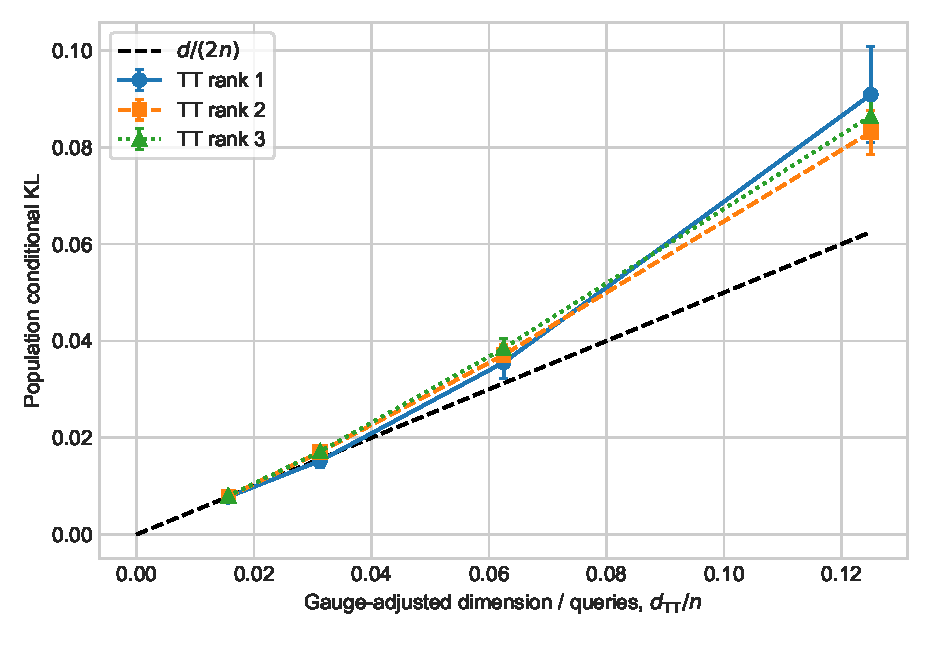
\includegraphics[width=.72\textwidth]{../figures/tt_rate.pdf}
\caption{Risks from all three TT ranks collapse when indexed by \(d_{TT}/n\). The black dashed line is the local asymptotic prediction \(d_{TT}/(2n)\); bars are pointwise 95\% Monte Carlo intervals, and marker/line shape identifies TT rank.}
\label{fig:tt-rate}
\end{figure}

Table~\ref{tab:geometry} verifies the quotient count exactly. At \(n/d=64\), the values of \(n\wh\cD/d\) are 0.497, 0.502, and 0.510 for ranks 1, 2, and 3. The average over all twelve conditions is 0.579; the excess above one half is concentrated in the smaller \(n/d\) conditions, as expected from finite-sample likelihood curvature. Figure~\ref{fig:tt-rate} shows that data from all three raw core counts collapse when indexed by the quotient dimension.

\subsection{Access-regime counterexample}

We next used \(d=20\). In the black-box experiment, the teacher was Bernoulli(1/2) and one response was sampled per prompt. In the exact-soft-label experiment, the value 1/2 was supplied as a fractional label. A misspecified soft-label condition used the nonlinear teacher
\[
q_0(1\mid X)=\operatorname{logit}^{-1}\left[
0.65\{\norm{X}^2-d\}/\sqrt{2d}\right]
\]
and a linear-logit student. Symmetry made the population projection zero, while prompt-specific gradients remained random.

\Cref{fig:access} compares the population excess risks under these three
observation regimes.

\begin{figure}[t]
\centering
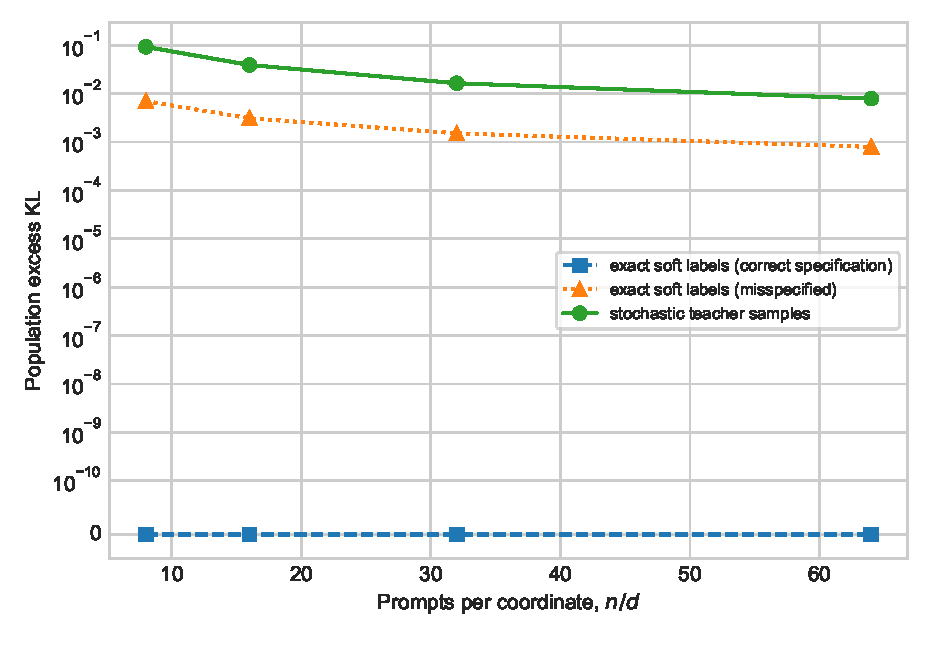
\includegraphics[width=.72\textwidth]{../figures/access_regimes.pdf}
\caption{The black-box risk decays at the usual parametric rate.  In this identifiable logistic example, exact soft labels recover the correctly specified parameter with zero numerical estimation error; the misspecified case has a smaller prompt-quadrature-dependent \(1/n\) term. The vertical scale is symmetric-log to display the exact zeros.}
\label{fig:access}
\end{figure}

With \(n/d=64\), \(n\wh\cD/d\) is 0.504 for stochastic responses, exactly zero to numerical precision for correctly specified soft labels, and 0.051 for misspecified soft labels. This instantiates the counterexample in \cref{prop:access}; it does not assert zero risk for every soft-label model. Under misspecification, the coefficient is determined by prompt-gradient variance rather than dimension alone.

\subsection{Functional misordering and a Gaussian benchmark}

For the explicit construction in \cref{prop:tt-misordering-paths}, we used the orthonormal rank-one TT atoms \(T_H=e_0^{\otimes4}\) and \(T_L=e_1^{\otimes4}\), amplitudes \(a=0.8\), \(b=1\), and scale \(t=0.5\). Both students have TT rank one and identical storage. Their Frobenius errors are 0.4 and 0.5, so reconstruction always selects \(A\). We then evaluated the exact Bernoulli KL, rather than substituting its quadratic expansion. As \(\rho_H/\rho_L\) ranges from 2 to 32, functional selection reduces exact population risk by factors 1.294 to 20.707; see \cref{fig:misordering-oracle}(a). The quadratic prediction, shown separately, is already close at this finite scale.

Finally, a separate Gaussian horizontal-coordinate experiment used candidate dimensions \(13,36,69,112\), the quotient dimensions of uniform-rank order-four TT models, and a polynomially decaying teacher. Mallows' unbiased criterion selected a truncation on the same observations. Over 3,000 replications, mean selected risk was between 1.023 and 1.102 times the infeasible minimum of approximation error plus \(d/n\); see \cref{fig:misordering-oracle}(b). This experiment illustrates the Gaussian-sequence benchmark in \cref{cor:scale}; because it fits neither TT cores nor a conditional generator, it does not validate the conditional-generator oracle in \cref{thm:oracle}.

\begin{figure}[t]
\centering
\begin{subfigure}{.48\textwidth}
\centering
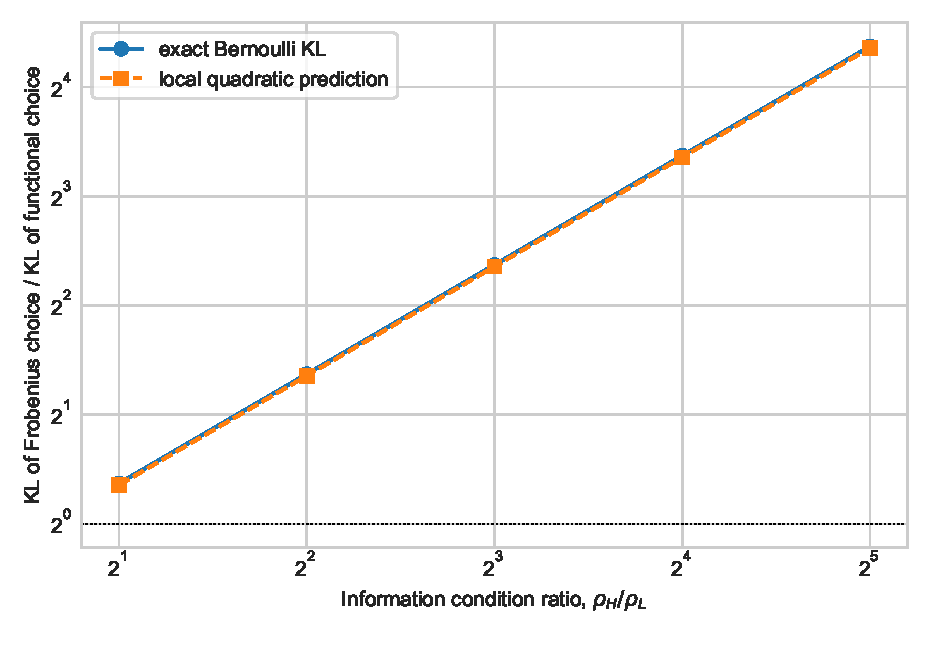
\includegraphics[width=\textwidth]{../figures/metric_misordering.pdf}
\caption{Metric misordering.}
\end{subfigure}\hfill
\begin{subfigure}{.48\textwidth}
\centering
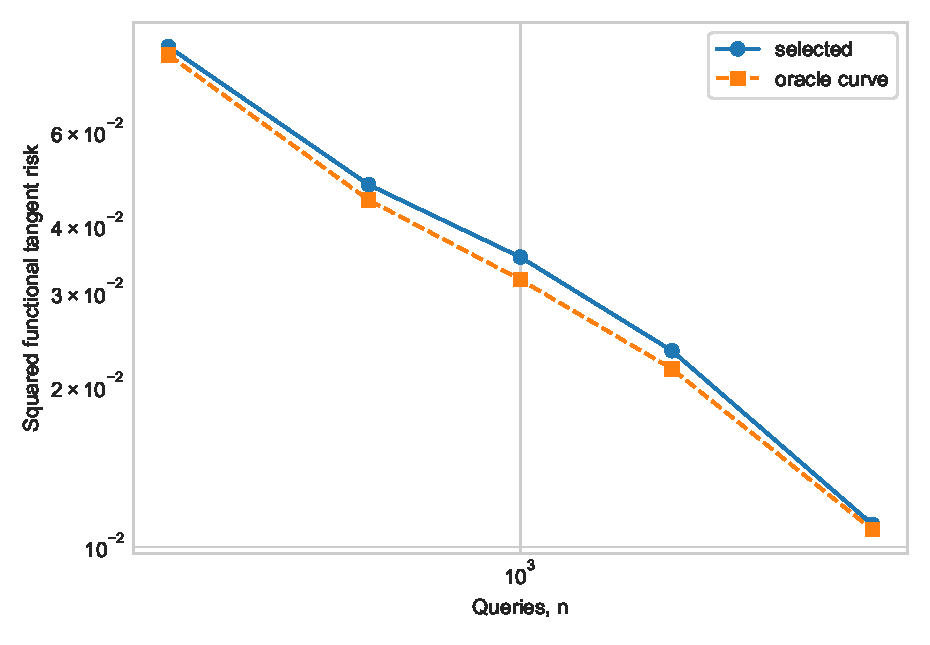
\includegraphics[width=\textwidth]{../figures/oracle_adaptation.pdf}
\caption{Gaussian selected versus benchmark risk.}
\end{subfigure}
\caption{Functional selection avoids a risk ratio that grows with metric anisotropy, while penalized coordinate selection stays close to its separate Gaussian-sequence benchmark. Panel (a) evaluates exact Bernoulli KL for two equal-budget rank-one TT students and overlays the local quadratic prediction; panel (b) averages 3,000 Gaussian-sequence replications at each \(n\) and is not a conditional-generator experiment.}
\label{fig:misordering-oracle}
\end{figure}

\subsection{Preregistered empirical falsification gate}

A subsequent open-model study should compare functional conditional-KL or Jacobian-pullback allocation against Frobenius, spectral, activation-reconstruction, and current loss-aware rank allocation on at least two model families. Ranks must be learned on calibration prompts and evaluated on held-out distributions and multiple capabilities. The theory-first direction should be abandoned or reframed if: (i) functional criteria do not improve held-out allocation ordering; (ii) the estimated functional information is effectively low rank and unstable across prompt resamples; or (iii) attainable optimizers cannot approach the oracle curve in a tractable frozen nonlinear block. This gate prevents the synthetic rate verification from being presented as evidence of LLM-scale benefit.

\section{Discussion}
\label{sec:discussion}

The main conclusion is conditional but sharp within its regular experiment. In a finite-query teacher experiment, a functionally identifiable TT quotient pays approximation error plus gauge-adjusted dimension over queries. A horizontal lower packing shows that the dimension term is not a proof artifact. Under the stated local information-normal and off-chart separation conditions, approximation and estimation are simultaneously unavoidable for a fixed compression class. The local constant depends on the relation between query and deployment information; \(d/2\) is the matched conditional-KL instance of the classical local asymptotic minimax calculation.

The access model can change the answer. White-box access to a feasible teacher gives zero risk immediately; exact soft labels also give finite-sample recovery in the identifiable logistic construction of \cref{prop:access}. These examples refute a universal positive \(d/n\) lower bound after the observation channel is changed, but they do not characterize the minimax rate of every soft-label experiment. Under misspecification, random deployment prompts create a quadrature term indexed by \(\tr(V_XH^{-1})\), which can be far smaller than \(d\) or zero. This distinction should influence practice: query-limited API distillation, finite Monte Carlo teacher sampling, exact soft-label distillation, and white-box tensorization should not automatically share one sample-complexity claim. Statistical explanations of soft-label variance reduction already appear in the distillation literature~\citep{phuong2019distillation,menon2021distillation,xie2026distillation}; our contribution is the access warning within the TT query experiment.

The gauge calculation is also insufficient by itself. It removes redundant core coordinates, but only restricted functional curvature makes all remaining tensor directions statistically visible. The results here cover the nondegenerate case in which the functional information is uniformly positive on the horizontal tangent. They do not prove a \(d_{\mathrm{fun}}/n\) law merely by replacing dimension with the rank of a singular pullback; weak eigenvalues and higher-order identification can produce different rates. Developing localized spectral complexity and adaptive penalties for weakly excited quotient directions is a natural next theoretical problem.

The rank-boundary result separates two goals that are often conflated. Penalized likelihood may adapt in prediction risk without consistently identifying a minimal rank. Honest rank identification requires functional separation from lower strata and, for consistency, a penalty stronger than an AIC-scale constant. The present two-point argument is generic; a TT-specific strengthening would relate functional separation quantitatively to the smallest relevant TT-unfolding singular values. A general theory over singular unions of TT varieties, rather than separated manifolds, would be required for a broader extension.

Same-data capability certification is useful only when the whole fitting map is stable. Its band is deliberately conservative and is an application of classical stability and bounded-differences arguments, not a new concentration principle~\citep{bousquet2002stability,feldman2019stability,bousquet2020sharper}. PAC--Bayes and protected-test methods already provide alternative simultaneous multi-risk guarantees~\citep{adams2024multiple,angelopoulos2021ltt,laufer2023pareto}. Cross-fitting, selective likelihood, or cluster jackknife methods may improve the adaptation price, but a final full-data refit creates a target mismatch that must be resolved rather than ignored. Protected-holdout Learn-then-Test remains preferable when nonconvex optimization has no stability guarantee.

Our literature search through 7 September 2026 supports a narrow priority statement, not proof of universal absence: among the primary sources examined, we did not identify a result simultaneously treating common TT-compressed weights inside a frozen nonlinear conditional generator, population teacher-relative conditional KL across environments, tensorization/rank selection in a finite stochastic-query experiment, and a local lower bound indexed by information on the TT gauge quotient. Tree-tensor risk oracles, TT minimax and inference, nonlinear low-rank neural rates, population/minimax KV-cache compression, statistical distillation, and Fisher- or KL-aware rank allocation already occupy each broader claim separately~\citep{michel2022tree,zhou2022ttoi,qin2024ttregression,arunan2026lora,haverbeck2026kvcache,menon2021distillation,iosvd2026,laser2026}. Our priority claim is therefore restricted to this coupling and to its explicit observation-model and functional-identifiability boundaries, rather than to any ingredient alone.

\paragraph{Limitations.}
The bounded likelihood-ratio assumption excludes unrestricted long-sequence log loss; the nonlinear verification covers a frozen block rather than every transformer layer; the statistical result assumes a global or certified approximate empirical optimizer; and the experiments are controlled tangent models rather than evidence from large open models. In addition, the leading oracle theorem is restricted to compact rank-separated strata and its constants can deteriorate with the atlas and smallest TT unfolding singular values. The joint approximation--estimation lower result constructs only a local information-normal tube and requires a separated off-chart complement. These are substantive limitations and define the next proof and empirical tasks.

\paragraph{Conclusion.}
We have formulated population functional risk as an explicit statistical target for query-limited TT compression and have shown why dimension-based guarantees require gauge quotienting, functional visibility, a fixed teacher access model, and controlled quotient charts. Under the stated regular, local information-normal, and off-chart separation conditions, the modelwise approximation--estimation frontier is sharp; outside them, local Fisher surrogates and \(d/n\) heuristics can be misleading.


\appendix
\section{Proofs for geometry and the oracle inequality}
\label{app:oracle-proofs}

\subsection{Elementary transfer and access results}

\begin{proof}[Proof of Proposition~\ref{prop:pinsker-transfer}]
Condition on \((X,R,E=e)\). The difference between expectations of a function with range length \(B_e\) under two probability measures is at most \(B_e\) times their total variation distance. Pinsker's inequality gives
\[
\TV(p_W,q_0)\le\sqrt{\KL(q_0\|p_W)/2}.
\]
Average over \((X,R)\), then use Jensen's inequality for the concave square root.
\end{proof}

\begin{proof}[Proof of Proposition~\ref{prop:access}]
For (i), returning the directly provided feasible parameter makes the student law equal
to the teacher law, so its population divergence is zero.

For (ii), strict monotonicity of the logistic link gives
\(\operatorname{logit}\{q_0(1\mid X_i)\}=X_i^\top\theta_0\).  A full-column-rank
design has the unique solution
\(\theta_0=(X^\top X)^{-1}X^\top z\), where
\(z_i=\operatorname{logit}\{q_0(1\mid X_i)\}\).  The recovered conditional law
therefore has zero population divergence.

For (iii), conditional cross-entropy decomposes pointwise as
\[
\bar\ell_\theta(x,e)=H\{q_0(\cdot\mid x,e)\}
+\KL\{q_0(\cdot\mid x,e)\|p_\theta(\cdot\mid x,e)\}.
\]
At correct specification, its gradient vanishes at \(\theta_0\) for every
prompt.  Under misspecification, the first-order condition and a Taylor
expansion give
\[
0=P_n\nabla\bar\ell_{\wh\theta}
=P_n\nabla\bar\ell_{\theta^*}
+H(\wh\theta-\theta^*)+o_p(n^{-1/2}).
\]
The multivariate central limit theorem yields the displayed sandwich limit. A second Taylor expansion of population risk gives
\[
\bar\cD_w(\wh\theta)-\bar\cD_w(\theta^*)
=\tfrac12(\wh\theta-\theta^*)^\top H(\wh\theta-\theta^*)
+o_p(n^{-1}).
\]
Taking expectations under uniform integrability and using cyclicity of trace yields
\[
\tfrac12\tr\{H(H^{-1}V_XH^{-1})\}
=\tfrac12\tr(V_XH^{-1}).
\]
At correct specification the pointwise gradient is zero, so \(V_X=0\). This is the standard smooth M-estimator calculation~\citep{vandervaart1998}.
\end{proof}

\subsection{TT geometry}

\begin{proof}[Proof of Lemma~\ref{lem:tt-dimension}]
For one layer, the product core space has dimension
\(m_\ell=\sum_jr_{\ell,j-1}m_{\ell j}r_{\ell j}\). Minimal TT representations of the same exact-rank tensor differ by the adjacent invertible transformations displayed in \cref{sec:geometry}; conversely these transformations preserve the contraction. On the minimal-rank stratum the action is free, so each orbit has dimension
\(\sum_{j<q_\ell}\dim\mathrm{GL}(r_{\ell j})
=\sum_{j<q_\ell}r_{\ell j}^2\). The quotient-manifold theorem therefore gives dimension \(m_\ell-\sum_{j<q_\ell}r_{\ell j}^2\)~\citep{holtz2012manifolds}. Independent layer products add dimensions, as do identifiable free coordinates. Tying imposes constraints across this product, so neither the product action nor the additive calculation need remain valid.
\end{proof}

\begin{proof}[Proof of Proposition~\ref{prop:tt-atlas}]
For any orthonormal basis \(U_{\ell j}\) of an unfolding column space,
Cauchy--Binet gives
\[
 1=\det(U_{\ell j}^\top U_{\ell j})
 =\sum_{|I|=r_{\ell j}}\det\{U_{\ell j}[I,:]\}^2.
\]
Consequently at least one row set \(I_{\ell j}\) has determinant in absolute
value at least \(c_{\ell j}\). Because every singular value of the square
submatrix is at most one, its smallest singular value is at least the absolute
determinant. Thus, for at least one pivot, the corresponding principal block
of the projector has smallest eigenvalue at least \(c_{\ell j}^2\). Every
tensor therefore belongs to the corresponding open patch with threshold
\(c_{\ell j}^2/4\) in \cref{eq:pivot-patch}. Counting pivot collections gives
\cref{eq:pivot-count}, including the separate atlas for constrained free
coordinates.

Write \(A=U_{\ell j}[I,:]\). On a thresholded patch, \(A\) is invertible and
\[
 P_{\ell j}[:,I]\{P_{\ell j}[I,I]\}^{-1}
 =U_{\ell j}A^\top(AA^\top)^{-1}
 =U_{\ell j}A^{-1}.
\]
Thus the normalized interface is expressed entirely through the column-space
projector and is independent of every choice of singular vectors. It fixes
the corresponding bond gauge uniquely, and \(\|A^{-1}\|_{\mathrm{op}}<
2/c_{\ell j}\) on the thresholded patch.

On the exact-minimal-rank core space, the derivative kernel of the full
contraction map is the vertical gauge tangent~\citep{holtz2012manifolds}.
Its restriction to the transverse normalized-pivot slice consequently has
zero kernel. Lemma~\ref{lem:tt-dimension} and the constant-rank theorem give
a \(d_\lambda\)-dimensional Euclidean chart around every point of a pivot
patch; they do not assert that the entire patch is one chart.

For uniform control, each unfolding has fixed rank and smallest nonzero
singular value at least \(\eta\). Its column-space spectral projector
\(P_{\ell j}\) is therefore \(C^2\) locally in the tensor, with derivatives
bounded in terms of \(\eta^{-1}\).
Sequential core recovery on a thresholded patch uses contractions, these
spectral projectors, pivot inverses bounded by \(2/c_{\ell j}\), and inverses
of nonzero unfolding blocks bounded by \(\eta^{-1}\). On the compact
\(R\)-bounded set, the quantitative constant-rank theorem therefore supplies
uniform local radii and the derivative bound in
\cref{eq:atlas-constant}. Compactness extracts finitely many such subcharts
over the finite pivot cover; their total number is \(H_\lambda\).

Finally, each subchart is \(C_{\mathrm{atlas},\lambda}\)-Lipschitz. Map the
standard Euclidean \(\epsilon/C_{\mathrm{atlas},\lambda}\)-net of a
\(d_\lambda\)-ball through the chart and use the volume bound
\(N(\delta,B_d(a,t),\norm{\cdot}_2)\le(1+2t/\delta)^{d_\lambda}\).
\end{proof}

\begin{proof}[Proof of Proposition~\ref{prop:block-curvature}]
Let \(S(p)=\operatorname{diag}(p)-pp^\top\). The logit derivative in direction \(H\) is
\[
D_Wz_W[H]=C\operatorname{diag}\{\phi'(Wh)\}Hh.
\]
The conditional softmax information quadratic form is
\[
\{D_Wz_W[H]\}^\top S(p_W)D_Wz_W[H].
\]
The assumed head and activation bounds make this at least
\(\kappa_C\kappa_\phi^2\norm{Hh}_2^2\). Averaging and using
\(\E(hh^\top)\succeq\kappa_hI\) gives
\[
\E\norm{Hh}_2^2=\tr\{H\E(hh^\top)H^\top\}
\ge\kappa_h\norm H_F^2.
\]
The result follows. The head condition also removes the softmax all-ones null direction.
\end{proof}

\subsection{Localized entropy and within-model fitting}

\begin{proof}[Proof of Lemma~\ref{lem:entropy}]
First suppose \(r<g_\lambda\). The global gap puts the entire risk sublevel inside \(U_\lambda^*\), and the margin places it in a Euclidean chart ball of radius \(\sqrt{2r/\mu_\lambda}\) about the projection representative. The pointwise likelihood Lipschitz condition maps a Euclidean \(\delta\)-net to an \(L_\infty\) net of radius at most \(L_\lambda\delta\). The standard volume cover of a \(d_\lambda\)-ball gives
\[
N(u\sqrt r,\mathcal F_\lambda(r),L_\infty)
\le
\left(1+\frac{2L_\lambda\sqrt{2/\mu_\lambda}}{u}\right)^{d_\lambda}.
\]
For \(r\ge g_\lambda\), cover the full compact atlas. If its largest coordinate diameter is \(R_\lambda\), the same argument gives
\[
N(u\sqrt r,\mathcal F_\lambda(r),L_\infty)
\le H_\lambda
\left(1+\frac{2L_\lambda R_\lambda}{u\sqrt{g_\lambda}}\right)^{d_\lambda}.
\]
These displays imply \cref{eq:local-entropy} after enlarging \(a_\lambda\).

Inside \(U_\lambda^*\), pointwise Lipschitzness and the margin give
\[
Q_0^w(\ell_W-\ell_{W_\lambda^*})^2
\le L_\lambda^2\norm{\theta-\theta_\lambda^*}^2
\le\frac{2L_\lambda^2}{\mu_\lambda}
\{\cD_w(W,W^0)-A_w^2(\lambda)\}.
\]
Outside that neighborhood, the likelihood difference is bounded by \(2B\) and the excess risk is at least \(g_\lambda\), which gives the factor \(4B^2/g_\lambda\). Compactness and continuity permit a finite enlargement of the constant on the interface.
\end{proof}

We record the empirical-process step used below. It is a localized finite-dimensional likelihood lemma, stated with the constants needed here.

\begin{lemma}[Localized likelihood deviation]
\label{lem:local-deviation}
Let \(\mathcal F\) be a pointwise measurable, separable, bounded loss-difference class with nonnegative means, variance bound \(Pf^2\le vPf\), and local uniform covering numbers
\[
\log N(u\sqrt r,\{f:Pf\le r\},L_\infty)
\le d\log(a/u)+h.
\]
There is \(C=C(a,v,\norm{\mathcal F}_\infty)\) such that, with probability at least \(1-e^{-z}\), simultaneously over \(f\in\mathcal F\),
\begin{equation}
|(P_n-P)f|\le\tfrac14Pf+C\frac{d+h+z}{n}.
\label{eq:isomorphic-lemma}
\end{equation}
The same conclusion holds for a finite atlas with the \(h=\log H\) term above.
\end{lemma}

\begin{proof}
We give the uniform-metric chaining step because an ordinary
\(L_2(P)\)-cover would not suffice. Fix \(r>0\), put
\(\mathcal F(r)=\{f:Pf\le r\}\), and take proper finite
\(L_\infty\)-nets \(T_k\subset\mathcal F(r)\), not necessarily nested, at radii
\(\epsilon_k=2^{-k}\sqrt r\), \(k\ge0\). Their logarithmic cardinalities are
at most
\[
 d\log(a2^k)+h.
\]
For a net point in \(T_0\), the variance is at most \(vr\) and its envelope
is at most \(\norm{\mathcal F}_\infty\). Bernstein's inequality and a union
bound control every such coarse point by
\[
 C\left\{\sqrt{\frac{vr(d+h+z)}n}
 +\frac{d+h+z}{n}\right\},
\]
where dependence on \(a\) and the envelope is absorbed into \(C\).

Let \(\pi_kf\) be a nearest point to \(f\) in \(T_k\), and connect these
approximants at adjacent levels. Every increment
\(\pi_kf-\pi_{k-1}f\) has envelope at most
\(3\epsilon_{k-1}\) and variance at most
\(9\epsilon_{k-1}^2\). Apply Bernstein simultaneously to all adjacent net
pairs, assigning level \(k\) failure probability proportional to
\(e^{-z-k}\). Summing the resulting bounds uses
\[
 \sum_{k\ge1}2^{-k}\sqrt{k+u}\le C\sqrt{1+u},
 \qquad
 \sum_{k\ge1}2^{-k}(k+u)\le C(1+u).
\]
Separability lets \(\pi_kf\to f\) uniformly. Consequently, with probability
at least \(1-e^{-z}\),
\begin{equation}
 \sup_{f\in\mathcal F(r)}|(P_n-P)f|
 \le C\left\{\sqrt{\frac{vr(d+h+z)}n}
 +\frac{d+h+z}{n}\right\}.
 \label{eq:local-chain-bound}
\end{equation}
The constant also absorbs the bounded uniform diameter in the linear
increment terms.

Finally apply \cref{eq:local-chain-bound} on the dyadic shells
\(2^{j-1}r_0<Pf\le2^jr_0\), assign shell \(j\) failure probability
proportional to \(e^{-z-j}\), and take
\(r_0=C_0(d+h+z)/n\). Young's inequality, together with
\(j+1\le2^{j+1}\), makes the square-root and shell-allocation terms at most
\(Pf/4+C(d+h+z)/n\) after increasing \(C_0\). The class is bounded, so only
finitely many nonempty shells are needed; the sublevel below \(r_0\) is
absorbed by the remainder. This proves \cref{eq:isomorphic-lemma}. It is the
standard localization-and-peeling scheme~\citep{koltchinskii2006local}, with
the uniform cover making the chaining valid for every empirical measure.
\end{proof}

Applying \cref{lem:local-deviation} to \(f_W=\ell_W-\ell_{W_\lambda^*}\), and using a weighted union bound with failure probability \(e^{-t}\pi_\lambda\), gives simultaneously over \(\lambda\)
\begin{equation}
\cD_w(\wh W_\lambda,W^0)-A_w^2(\lambda)
\le C_{\mathrm{reg},\lambda}
\frac{d_\lambda+\log H_\lambda+x_\lambda+t}{n_1}
+C\varepsilon_{\lambda,\mathrm{opt}}.
\label{eq:within-rate}
\end{equation}
Indeed, insert the approximate ERM inequality into two copies of \cref{eq:isomorphic-lemma} and absorb the quarter-risk terms.

\subsection{Validation selection and proof of the oracle}

\begin{lemma}[Likelihood-ratio Bernstein condition]
\label{lem:lr-bernstein}
If \(u=p_W/q_0\in[e^{-B},e^B]\), then
\[
Q_0^w\left\{\log(q_0/p_W)\right\}^2
\le c_B\cD_w(W,W^0),
\quad
c_B=\sup_{u\in[e^{-B},e^B]}
\frac{(\log u)^2}{u-1-\log u}<\infty.
\]
\end{lemma}

\begin{proof}
Conditional on \((X,E)\), \(\E_{q_0}(u-1)=0\), and hence
\[
\KL(q_0\|p_W)=\E_{q_0}\{u-1-\log u\}.
\]
The scalar ratio defining \(c_B\) extends continuously at \(u=1\), with limit 2, and is bounded on the compact interval. Integrate the scalar inequality and then average over prompts.
\end{proof}

\begin{proof}[Proof of Theorem~\ref{thm:oracle}]
Condition on the training split. Then \(\wh W_\lambda\) is fixed for validation. Bernstein's inequality, Lemma~\ref{lem:lr-bernstein}, and the inequality \(2\sqrt{ab}\le a/4+4b\) imply, with conditional probability at least \(1-e^{-t}\), simultaneously over \(\lambda\),
\begin{equation}
\left|(P_{n_2}-P_0)h_\lambda\right|
\le\tfrac14P_0h_\lambda+C_B\frac{x_\lambda+t}{n_2},
\quad h_\lambda=\log(q_0/p_{\wh W_\lambda}).
\label{eq:validation-deviation}
\end{equation}
Here the weighted union bound uses \(\sum_\lambda\pi_\lambda\le1\). The unknown term \(-\log q_0\) cancels from the empirical comparison in \cref{eq:selector}, so the selector also compares \(P_{n_2}h_\lambda\).

For any comparator \(\lambda\), combine the lower side of \cref{eq:validation-deviation} for \(\wh\lambda\), the selection inequality, and the upper side for \(\lambda\):
\begin{align*}
\tfrac34\cD_w(\wh W,W^0)
&\le P_{n_2}h_{\wh\lambda}
+C_B\frac{x_{\wh\lambda}+t}{n_2}\\
&\le P_{n_2}h_\lambda
+\kappa_B\frac{x_\lambda-x_{\wh\lambda}}{n_2}
+\varepsilon_{\mathrm{sel}}
+C_B\frac{x_{\wh\lambda}+t}{n_2}\\
&\le\tfrac54\cD_w(\wh W_\lambda,W^0)
+C_B\frac{x_\lambda+t}{n_2}
+\kappa_B\frac{x_\lambda-x_{\wh\lambda}}{n_2}
+C_B\frac{x_{\wh\lambda}+t}{n_2}
+\varepsilon_{\mathrm{sel}}.
\end{align*}
Choose \(\kappa_B\ge C_B\) and enlarge constants; the selected-index code term is nonpositive after cancellation. Insert \cref{eq:within-rate}, then take the infimum over \(\lambda\), proving \cref{eq:oracle-hp}.

Under uniform regularity and balanced splits, integrate the exponential tail. Bounded risk controls the small-probability complement and contributes at most \(C/n\) after a standard truncation of the tail integral. This proves \cref{eq:oracle-expectation}.
\end{proof}

\begin{proof}[Proof of Corollary~\ref{cor:same-sample-oracle}]
Subtract the unavailable but candidate-independent empirical teacher log likelihood from the penalized criterion. Apply the assumed isomorphic inequality to the selected candidate and to an arbitrary comparator. A sufficiently large penalty cancels the selected model's complexity; absorb the two quarter-risk terms and optimize over the comparator.
\end{proof}

\section{Proofs of lower and adaptation results}
\label{app:lower-proofs}

\begin{proof}[Proof of Theorem~\ref{thm:lower}]
Let \(\omega\in\{-1,1\}^d\) and set \(u_\omega=a\omega\), where
\[
a^2=c_0\left(\frac1n\wedge\frac{\rho^2}{d}\right)
\]
and \(c_0\) is sufficiently small. Then \(u_\omega\in B_d(0,\rho)\). If \(\omega\) and \(\omega^{(j)}\) differ only in coordinate \(j\), \cref{eq:kl-upper} gives
\[
\KL\{(Q_{u_\omega}^w)^{\otimes n}\|
        (Q_{u_{\omega^{(j)}}}^w)^{\otimes n}\}
\le 4C_Kna^2\le4C_Kc_0.
\]
Choose \(c_0\) so that Pinsker's inequality bounds the total variation between every neighboring product experiment by at most \(1/2\). Assouad's lemma then forces expected Hamming error at least \(d/4\) for any decoder of \(\omega\).

Given an arbitrary estimated conditional distribution \(\wt p\), let
\(\wh\omega\) be a Hellinger-nearest vertex, with measurable tie breaking.
Because \(p_{u_\omega}\) is one of the vertices, the triangle inequality gives
\[
h_w(p_{u_\omega},p_{u_{\wh\omega}})
\le 2h_w(p_{u_\omega},\wt p).
\]
Together with \cref{eq:hell-lower}, this implies
\[
h_w^2(p_{u_\omega},\wt p)
\ge c_h a^2d_H(\omega,\wh\omega),
\]
where \(d_H\) is Hamming distance. Therefore
\[
\sup_\omega\E_\omega h_w^2(p_{u_\omega},\wt p)
\ge c d a^2
=c\left(\rho^2\wedge\frac dn\right).
\]
Finally \(\Kw{q}{p}\ge h_w^2(q,p)\) under the convention
\(h^2=\int(\sqrt q-\sqrt p)^2\), which proves the claim. See~\citet{tsybakov2009} for the metric form of Assouad's lemma.
\end{proof}

\begin{proof}[Proof of Proposition~\ref{prop:normal-tube}]
To verify the asserted local existence of the normal field, choose a nonzero
vector \(v_0\) in the \(J_w\{\iota(0)\}\)-orthogonal complement of
\(D\iota(0)\). The matrices
\[
\Pi_u=I_D-D\iota(u)
\{D\iota(u)^\top J_w(\iota(u))D\iota(u)\}^{-1}
D\iota(u)^\top J_w(\iota(u))
\]
project onto the corresponding information-normal spaces. For the sufficiently
small \(\rho_0\) fixed in the proposition, \(\Pi_uv_0\) stays nonzero;
normalizing it in the \(J_w\)-metric
produces a \(C^2\) field satisfying \cref{eq:fisher-normal}. Compactness of
the smaller closed ball supplies the derivative bounds, and openness of
\(\mathcal U\) ensures \(\iota(u)+aN(u)\in\mathcal U\) for small \(a\).

The common-support and dominated-derivative assumptions give the uniform
two-parameter KL expansion
\begin{equation}
\Kw{p_\zeta}{p_{\zeta'}}
=\tfrac12(\zeta'-\zeta)^\top
J_w(\zeta_0)(\zeta'-\zeta)
+R(\zeta,\zeta';\zeta_0),
\qquad
|R|\le C(\norm{\zeta-\zeta_0}+\norm{\zeta'-\zeta_0})^3,
\label{eq:two-parameter-kl-expansion}
\end{equation}
whenever all three parameters lie in a sufficiently small common
neighborhood. This follows by differentiating KL in both arguments at
\((\zeta_0,\zeta_0)\): both first derivatives vanish and the second-order
quadratic form is the information applied to the parameter difference.

Take \(\zeta_0=\iota(u)\), \(\zeta=\zeta_{u,a}\), and
\(\zeta'=\iota(v)\). Taylor expansion of the embedding gives
\[
\zeta'-\zeta
=D\iota(u)(v-u)-aN(u)+O(\norm{v-u}^2).
\]
The cross term in the leading quadratic vanishes by
\cref{eq:fisher-normal}; information nondegeneracy and the singular-value
bounds for \(D\iota\) make the remaining quadratic uniformly equivalent to
\(a^2+\norm{u-v}^2\). The initial choice of \(\rho_0\), followed by shrinking
\(a_0\), absorbs the cubic
remainder and proves both sides of \cref{eq:tube-loss}.

The map \(u\mapsto\zeta_{u,a}\) has a uniformly bounded derivative. Applying
the upper side of \cref{eq:two-parameter-kl-expansion} to
\(p_{\zeta_{u,a}}\) and \(p_{\zeta_{v,a}}\) therefore gives
\[
\Kw{P_{u,a}}{P_{v,a}}\le C_T\norm{u-v}^2.
\]
The environment--prompt marginal is common, so this conditional KL equals
the one-observation joint KL; product additivity proves
\cref{eq:tube-kl}.

For the approximation statement, the candidate \(p_{\iota(u)}\) and the
upper side of \cref{eq:tube-loss} give
\(A_w^2(\lambda;P_{u,a})\le C_Ta^2\). The lower side gives
\(c_Ta^2\) for every candidate in the local chart. Shrink \(a_0\) further so
that \(c_Ta_0^2\le g_0\);
\cref{eq:off-chart-gap} excludes every remaining candidate and proves the
lower side of \cref{eq:tube-approx}.
\end{proof}

\begin{proof}[Proof of Theorem~\ref{thm:tube-lower}]
Put a hypercube \(u_\omega=\delta\omega\) in \(B_d(0,\rho)\), where
\[
\delta^2=c_0\left(\frac1n\wedge\frac{\rho^2}{d}\right).
\]
By \cref{eq:tube-kl}, neighboring product experiments have KL at most a
fixed constant when \(c_0\) is sufficiently small. Hence Assouad's lemma
forces Hamming error of order \(d\).

If \(\wt W\) lies in the local chart, write
\(\wt W=\iota(\wh v)\). If it lies outside, set \(\wh v=0\). In the first
case \cref{eq:tube-loss} gives
\[
\Kw{P_{u_\omega,a}}{p_{\wt W}}
\ge c_Ta^2+c_T\norm{u_\omega-\wh v}^2.
\]
In the second case, \cref{eq:off-chart-gap}, together with the choice of the
small local radii, bounds the same loss below by a sufficiently small constant
multiple of \(a^2+\norm{u_\omega-\wh v}^2\). Decode a nearest hypercube
vertex from \(\wh v\). The Euclidean version of the nearest-vertex argument
in the proof of Theorem~\ref{thm:lower} and Assouad's lemma give
\[
\sup_\omega\E_{u_\omega,a}
\Kw{P_{u_\omega,a}}{p_{\wt W}}
\ge ca^2+cd\delta^2.
\]
Since the hypercube is a subset of the ball, this is
\cref{eq:tube-lower-result}.
\end{proof}

\begin{proof}[Proof of Proposition~\ref{cor:scale}]
For a fixed integer \(D\), the truncation estimator
\(\wh\theta_j=Z_j\mathbf 1\{j\le D\}\) has risk
\[
\frac Dn+\sum_{j>D}\theta_j^2
\le \frac Dn+L^2D^{-2s}.
\]
Taking the best \(D\) proves the upper bound.

For the lower bound, first suppose the variance--bias crossing occurs at an
integer \(D\ge1\), up to a constant factor depending only on \(s\):
\[
D/n\asymp L^2D^{-2s}.
\]
Place a hypercube on the shell \(j=D+1,\ldots,2D\), with each active
coordinate equal to \(\pm\delta\), where
\[
\delta^2=c_s\min\left\{\frac1n,
L^2D^{-(2s+1)}\right\}.
\]
For sufficiently small \(c_s\), every vertex belongs to
\(\mathcal H_s(L)\): if \(m\le D\), its tail energy is at most
\(D\delta^2\le L^2D^{-2s}\le L^2m^{-2s}\); if
\(D<m<2D\), use \(m^{-2s}\ge(2D)^{-2s}\) and decrease \(c_s\); for
\(m\ge2D\) the tail is zero. Neighboring Gaussian experiments have KL
\(2n\delta^2\), which is bounded by a sufficiently small constant.
Assouad's lemma therefore yields risk at least
\[
cD\delta^2
\asymp c_s\left\{D/n+L^2D^{-2s}\right\},
\]
where the final equivalence uses the crossing relation. Monotonicity of the
two terms shows that this is within a constant factor of their infimum.

If the continuous crossing lies below one, then \(L^2<1/n\) and the displayed
infimum is comparable to \(1/n\). A two-point experiment in the unconstrained
first coordinate, at separation \(c/\sqrt n\), gives this lower bound.
Rounding the crossing to an integer changes constants only. The bounded-ratio
grid statement follows by rounding \(D\) upward to the next grid point.
\end{proof}

\begin{proof}[Proof of Theorem~\ref{thm:lan}]
Differentiability in quadratic mean and nonsingular \(I_\pi\) imply convergence of the local experiments to the Gaussian shift
\[
Z=h+I_\pi^{-1/2}\xi,\qquad \xi\sim N(0,I_d).
\]
For every \(M<\infty\), apply the local asymptotic minimax theorem to the
bounded bowl-shaped loss
\[
\ell_M(a,h)=\min\{M,\tfrac12(a-h)^\top G_w(a-h)\}.
\]
The assumed uniform truncated-loss convergence and coercivity justify the
transfer from the original estimator range to the local Gaussian experiment
\citep{vandervaart1998}. Letting the local ball expand and then
\(M\to\infty\), monotone convergence gives the minimax risk of the untruncated
Gaussian shift. The equivariant estimator \(\wh h=Z\) has risk
\[
\tfrac12\E\xi^\top I_\pi^{-1/2}G_wI_\pi^{-1/2}\xi
=\tfrac12\tr(G_wI_\pi^{-1}),
\]
and is minimax in the expanding-ball limit. An asymptotically linear efficient
estimator, uniformly on compact local alternatives, attains the same constant
when its rescaled losses are uniformly integrable. At correct conditional
specification, the target Hessian is \(I_w\); setting \(w=\pi\) gives
\(\tr(I_d)/2=d/2\).
\end{proof}

\begin{proof}[Proof of Proposition~\ref{prop:misspecified-constant}]
The asserted asymptotic linearity and central limit theorem give covariance
\[
\Sigma_\pi=H_\pi^{-1}V_\pi H_\pi^{-1}
\]
for \(\sqrt n(\wh\theta-\theta^*)\). Because \(\theta^*\) is stationary, a
second-order expansion of the target risk gives
\[
R_w(\wh\theta)-R_w(\theta^*)
=\tfrac12(\wh\theta-\theta^*)^\top
G_w(\wh\theta-\theta^*)+o_p(n^{-1}).
\]
Uniform integrability permits expectations to pass through this expansion.
The Gaussian quadratic-form identity and cyclicity of trace then yield
\[
\lim_{n\to\infty}n\E\{R_w(\wh\theta)-R_w(\theta^*)\}
=\tfrac12\tr(G_w\Sigma_\pi)
=\tfrac12\tr\{G_wH_\pi^{-1}V_\pi H_\pi^{-1}\}.
\]
\end{proof}

\begin{proof}[Proof of Theorem~\ref{thm:rank-impossibility}]
Any rank selector induces a test between \(W_0\) and \(W_t\): accept the higher-rank alternative when it returns \(\bm r\). The larger of its two rank errors is at least half the sum of the two testing errors. The optimal sum is
\(1-\TV\{(Q_{W_0}^\pi)^{\otimes n},(Q_{W_t}^\pi)^{\otimes n}\}\). By product additivity of KL and Pinsker's inequality,
\[
\TV\{(Q_{W_0}^\pi)^{\otimes n},(Q_{W_t}^\pi)^{\otimes n}\}
\le\sqrt{\frac n2\KL(Q_{W_0}^\pi\|Q_{W_t}^\pi)}
\le\sqrt{Cn\delta_t^2/2}.
\]
Substitution proves the result.
\end{proof}

\begin{proof}[Proof of Proposition~\ref{prop:rank-sufficiency}]
The criterion of the true rank is at most
\(P_n\ell_W+\operatorname{pen}_{\bm r}/n\). On the asserted event, every
underfit criterion exceeds this upper bound by at least
\[
g_n/2+(\operatorname{pen}_{\bm s}-
\operatorname{pen}_{\bm r})/n>0,
\]
and every overfit criterion exceeds it by at least
\[
(\operatorname{pen}_{\bm s}-\operatorname{pen}_{\bm r}
-b_{\bm s,n})/n>0.
\]
Thus \(\wh{\bm r}=\bm r\) on events whose probabilities tend to one.
\end{proof}

\section{Proofs for functional selection and certification}
\label{app:secondary-proofs}

\begin{proof}[Proof of Theorem~\ref{thm:misordering}]
Generalized eigenvector normalization gives
\[
v_H^\top Qv_H=v_L^\top Qv_L=1,
\quad v_H^\top G_w(W_*)v_H=\lambda_H,
\quad v_L^\top G_w(W_*)v_L=\lambda_L.
\]
Therefore the two reconstruction errors are \(t^2a^2+O(t^3)\) and \(t^2b^2+O(t^3)\), respectively. Since \(a<b\), the first is smaller for sufficiently small \(t\). Continuity of the pullback as \(W^0(t)\to W_*\) and a uniform Taylor expansion about the moving teacher give functional risks
\(t^2\lambda_Ha^2/2+o(t^2)\) and
\(t^2\lambda_Lb^2/2+o(t^2)\). Their assumed strict inequality survives for small \(t\). Taking \(a^2/b^2\uparrow1\) makes the risk ratio approach \(\lambda_H/\lambda_L\).
\end{proof}

\begin{proof}[Proof of Proposition~\ref{prop:tt-misordering-paths}]
Both students are scalar multiples of rank-one TT tensors and hence have the
same TT ranks and parameter count.  Their squared Frobenius errors are
\(t^2a^2\) and \(t^2b^2\).  At \(W=0\), the Bernoulli logistic information
quadratic form restricted to \(\operatorname{span}(T_H,T_L)\) is
\[
 G_0[U,U]=\tfrac14\E\langle U,X\rangle^2,
\]
so its eigenvalues in these two orthonormal directions are
\(\rho_H/4\) and \(\rho_L/4\).  A third-order Taylor expansion of
teacher-relative conditional KL, uniformly along the two finite-dimensional
paths, therefore gives
\[
 \cD_w\{W_A(t);W^0(t)\}=\frac{t^2\rho_Ha^2}{8}+O(t^3),\qquad
 \cD_w\{W_B(t);W^0(t)\}=\frac{t^2\rho_Lb^2}{8}+O(t^3).
\]
The two strict inequalities follow from \(a<b\) and
\(\rho_Ha^2>\rho_Lb^2\).
\end{proof}

\begin{proof}[Proof of Corollary~\ref{cor:selection-gap}]
Let \(V_i=\ell_{W_A}(Z_i)-\ell_{W_B}(Z_i)\). Then \(\E V_i=\gamma\), and the likelihood-ratio bound implies \(V_i\in[-2B,2B]\). Functional validation makes an error only if \(n_2^{-1}\sum_iV_i\le0\). Hoeffding's inequality gives probability at most
\(\exp\{-2n_2\gamma^2/(4B)^2\}=\exp\{-n_2\gamma^2/(8B^2)\}\).
\end{proof}

\begin{proof}[Proof of Theorem~\ref{thm:certificate}]
Fix \((e,\lambda)\) and abbreviate \(A=\mathsf A_\lambda\), \(H=H_e\), \(\beta=\beta_{e\lambda}\), and \(M=M_e\). Define the generalization gap
\[
F(S)=\E_C H\{A(S);C\}-G^{-1}\sum_{g=1}^G H\{A(S);C_g\}.
\]
The replace-one argument for uniform stability gives \(|\E F(S)|\le\beta\). If one cluster in \(S\) is replaced, the population term changes by at most \(\beta\). In the empirical term, the \(G-1\) unchanged evaluations each change by at most \(\beta\), and the replaced evaluation changes by at most \(M\). Hence the bounded-difference constant is at most
\[
\beta+\frac{(G-1)\beta+M}{G}\le2\beta+M/G.
\]
Two applications of McDiarmid's inequality therefore give, with probability at least \(1-\delta\),
\[
|F(S)|\le\beta+(2G\beta+M)
\sqrt{\frac{\log(2/\delta)}{2G}}.
\]
Set \(\delta=\alpha\pi_\lambda/K\) and union-bound over \(e\) and \(\lambda\). Since \(\sum_\lambda\pi_\lambda\le1\), the total failure probability is at most \(\alpha\), proving \cref{eq:sim-band}.
\end{proof}

\begin{proof}[Proof of Corollary~\ref{cor:strong-convex-stability}]
Let \(\wh\theta_S,\wh\theta_{S'}\) minimize the two objectives. Add their strong-convexity optimality inequalities. All common empirical summands cancel, and Lipschitzness of the one replaced summand yields
\[
\mu\norm{\wh\theta_S-\wh\theta_{S'}}^2
\le\frac{2L}{G}\norm{\wh\theta_S-\wh\theta_{S'}},
\]
so their distance is at most \(2L/(\mu G)\). Evaluation-loss Lipschitzness then gives
\(\beta\le2L^2/(\mu G)\), the standard regularized-ERM stability calculation~\citep{bousquet2002stability}.
\end{proof}

\section{Reproducibility details and additional numerical results}
\label{app:experiments}

All experiments use NumPy/SciPy pseudorandom generator seed 20260907. TT contractions use double precision. The core-to-tensor Jacobian is computed by centered differences with step \(10^{-6}\); its numerical-rank threshold is \(10^{-8}\) times the largest singular value. The smallest retained singular values for TT ranks 1, 2, and 3 are 0.370, 0.069, and 0.027, while gauge-null singular values are below \(10^{-9}\).

Bernoulli likelihoods are optimized by damped Newton steps with backtracking and a \(10^{-9}\) numerical ridge. Population KL is evaluated on a common 12,000-prompt test design within each TT rank. The exact-soft-label experiment uses 30,000 test prompts. The separate Gaussian-sequence benchmark has ambient dimension 180, candidate quotient dimensions \(13,36,69,112\), coefficient sequence
\(\theta_j=1.4j^{-1.3}\), and the criterion
\[
\operatorname{Crit}(d)=\sum_{j>d}Z_j^2+2d/n.
\]
The additive term independent of \(d\) is omitted.  The metric-misordering
experiment uses \(T_H=e_0^{\otimes4}\), \(T_L=e_1^{\otimes4}\),
\((a,b,t)=(0.8,1,0.5)\), and exact Bernoulli KL under
\(\rho_H/\rho_L\in\{2,4,8,16,32\}\).  Both candidate tensors have TT rank
one; the local quadratic risks in the plot are reference values, not the
simulated target.

Full TT-tangent risks and Gaussian-sequence selection summaries appear in
\cref{tab:rate-full,tab:oracle-full}, respectively.

\begin{table}[ht]
\centering
\caption{Normalized TT-tangent risk \(n\wh\cD/d\). Values tend toward the LAN constant \(1/2\).}
\label{tab:rate-full}
\begin{tabular}{rcccc}
\toprule
& \multicolumn{4}{c}{\(n/d\)}\\
TT rank & 8 & 16 & 32 & 64\\
\midrule
1 & 0.727 & 0.569 & 0.487 & 0.497\\
2 & 0.665 & 0.594 & 0.545 & 0.502\\
3 & 0.692 & 0.616 & 0.549 & 0.510\\
\bottomrule
\end{tabular}
\end{table}

\begin{table}[ht]
\centering
\caption{Gaussian-sequence model selection. The ratio compares mean selected risk with the approximation-plus-estimation benchmark.}
\label{tab:oracle-full}
\begin{tabular}{rrrrr}
\toprule
\(n\) & Oracle \(d\) & Mean selected \(d\) & Oracle risk & Risk ratio\\
\midrule
200  & 13 & 13.32 & 0.0837 & 1.036\\
500  & 13 & 14.23 & 0.0447 & 1.068\\
1000 & 13 & 18.02 & 0.0317 & 1.102\\
2000 & 36 & 29.17 & 0.0216 & 1.081\\
5000 & 36 & 37.08 & 0.0108 & 1.023\\
\bottomrule
\end{tabular}
\end{table}

The script \texttt{code/run\_simulations.py} regenerates every table source and figure. The \texttt{--quick} flag reduces Monte Carlo counts without altering conditions; \texttt{code/test\_simulations.py} checks the dimension formula, KL implementation, and exact-soft-label optimizer.


\bibliographystyle{plainnat}
\bibliography{references}
\end{document}
